\section{機能ごとのモジュール設計}
この先,時間の都合上フロー図はない.

\vspace{-0.5cm}
%曲名.作曲者・編曲者検索
\subsection*{楽譜を曲名,作曲者・編曲者,グレードから検索する機能}
検索ボックス,プルダウンへの入力値を受け取り,その文字列を曲名に含むデータ,または
作曲者・編曲者・グレードに含むデータを検索する.
\begin{figure}[H]
    \centering
    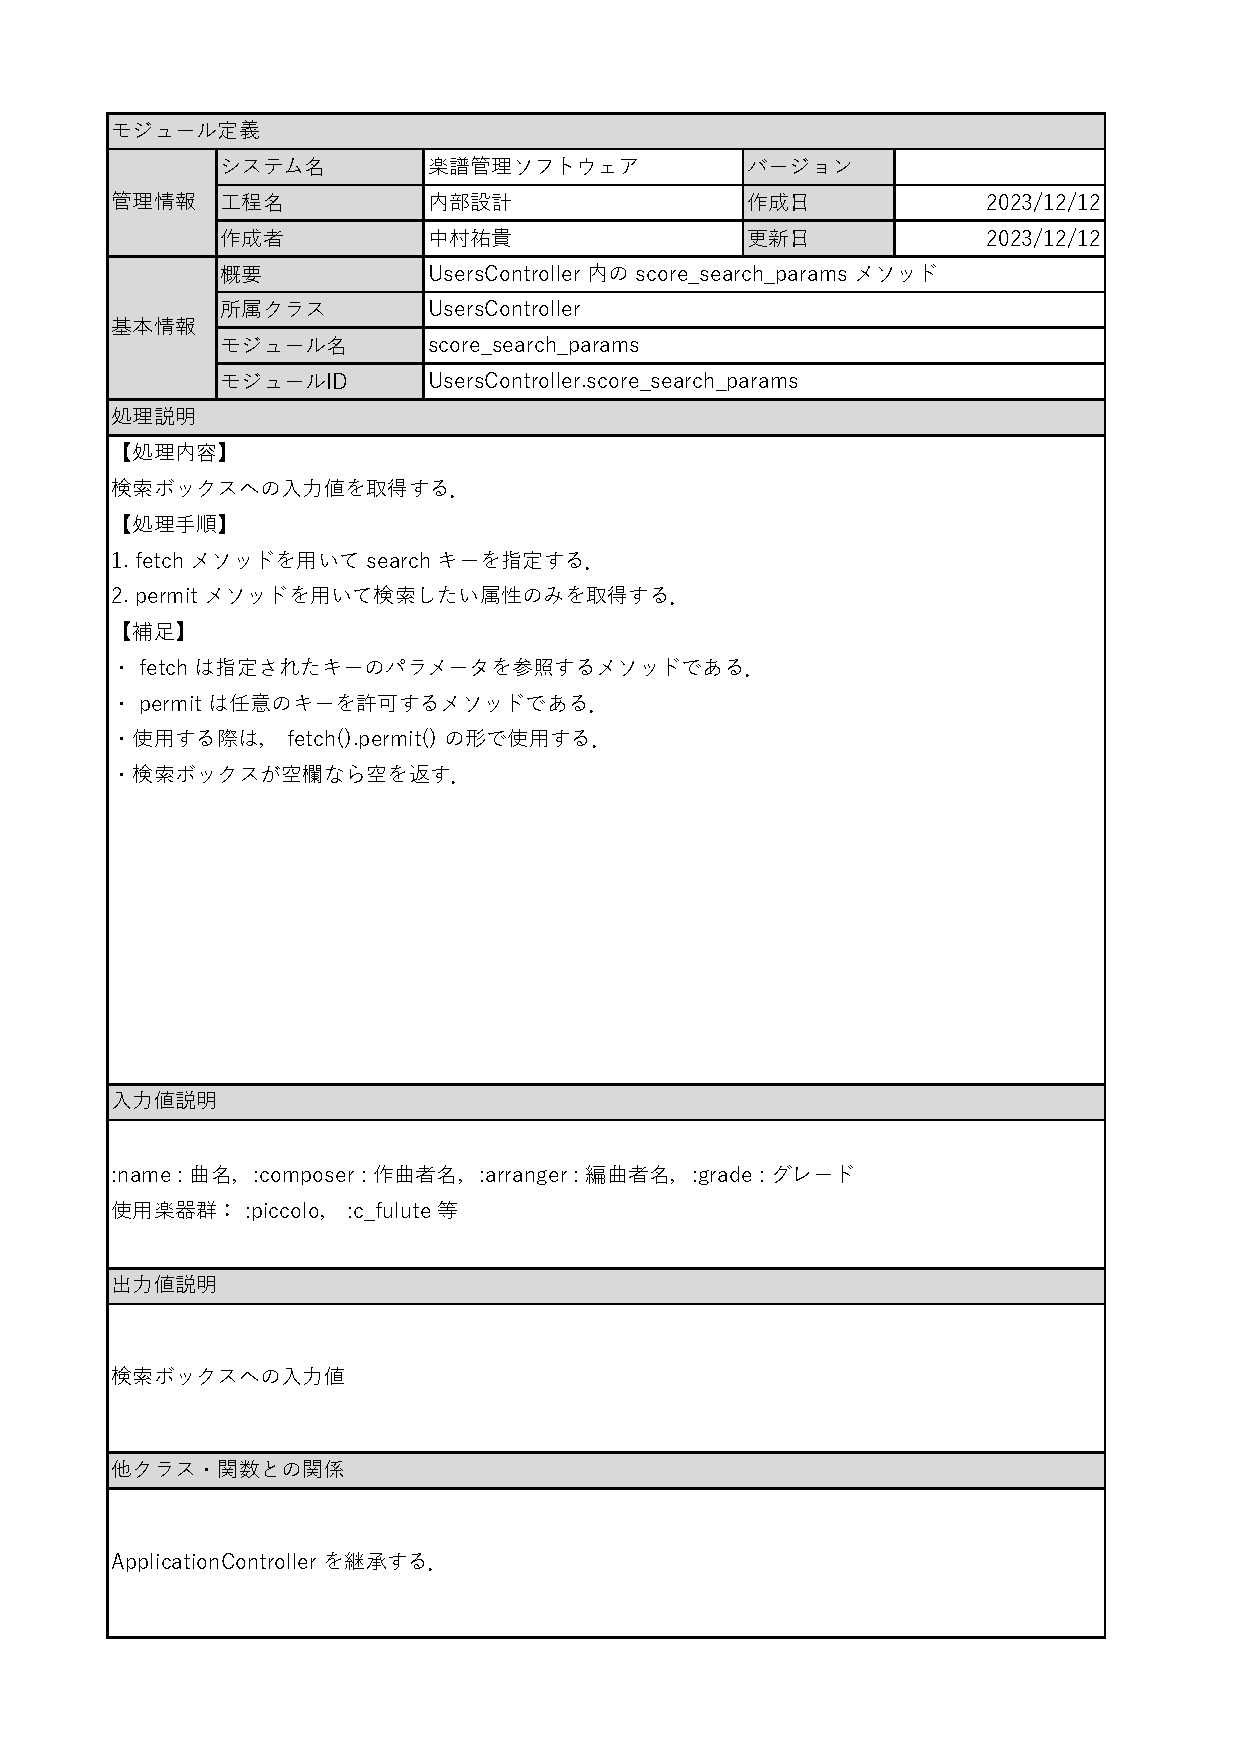
\includegraphics[scale=0.5]{img/Method/score_search_params}
    \caption{ScoresController.score\_search\_params}
    \label{ScoresController.score-search-params}
\end{figure}
\begin{figure}
    \centering
    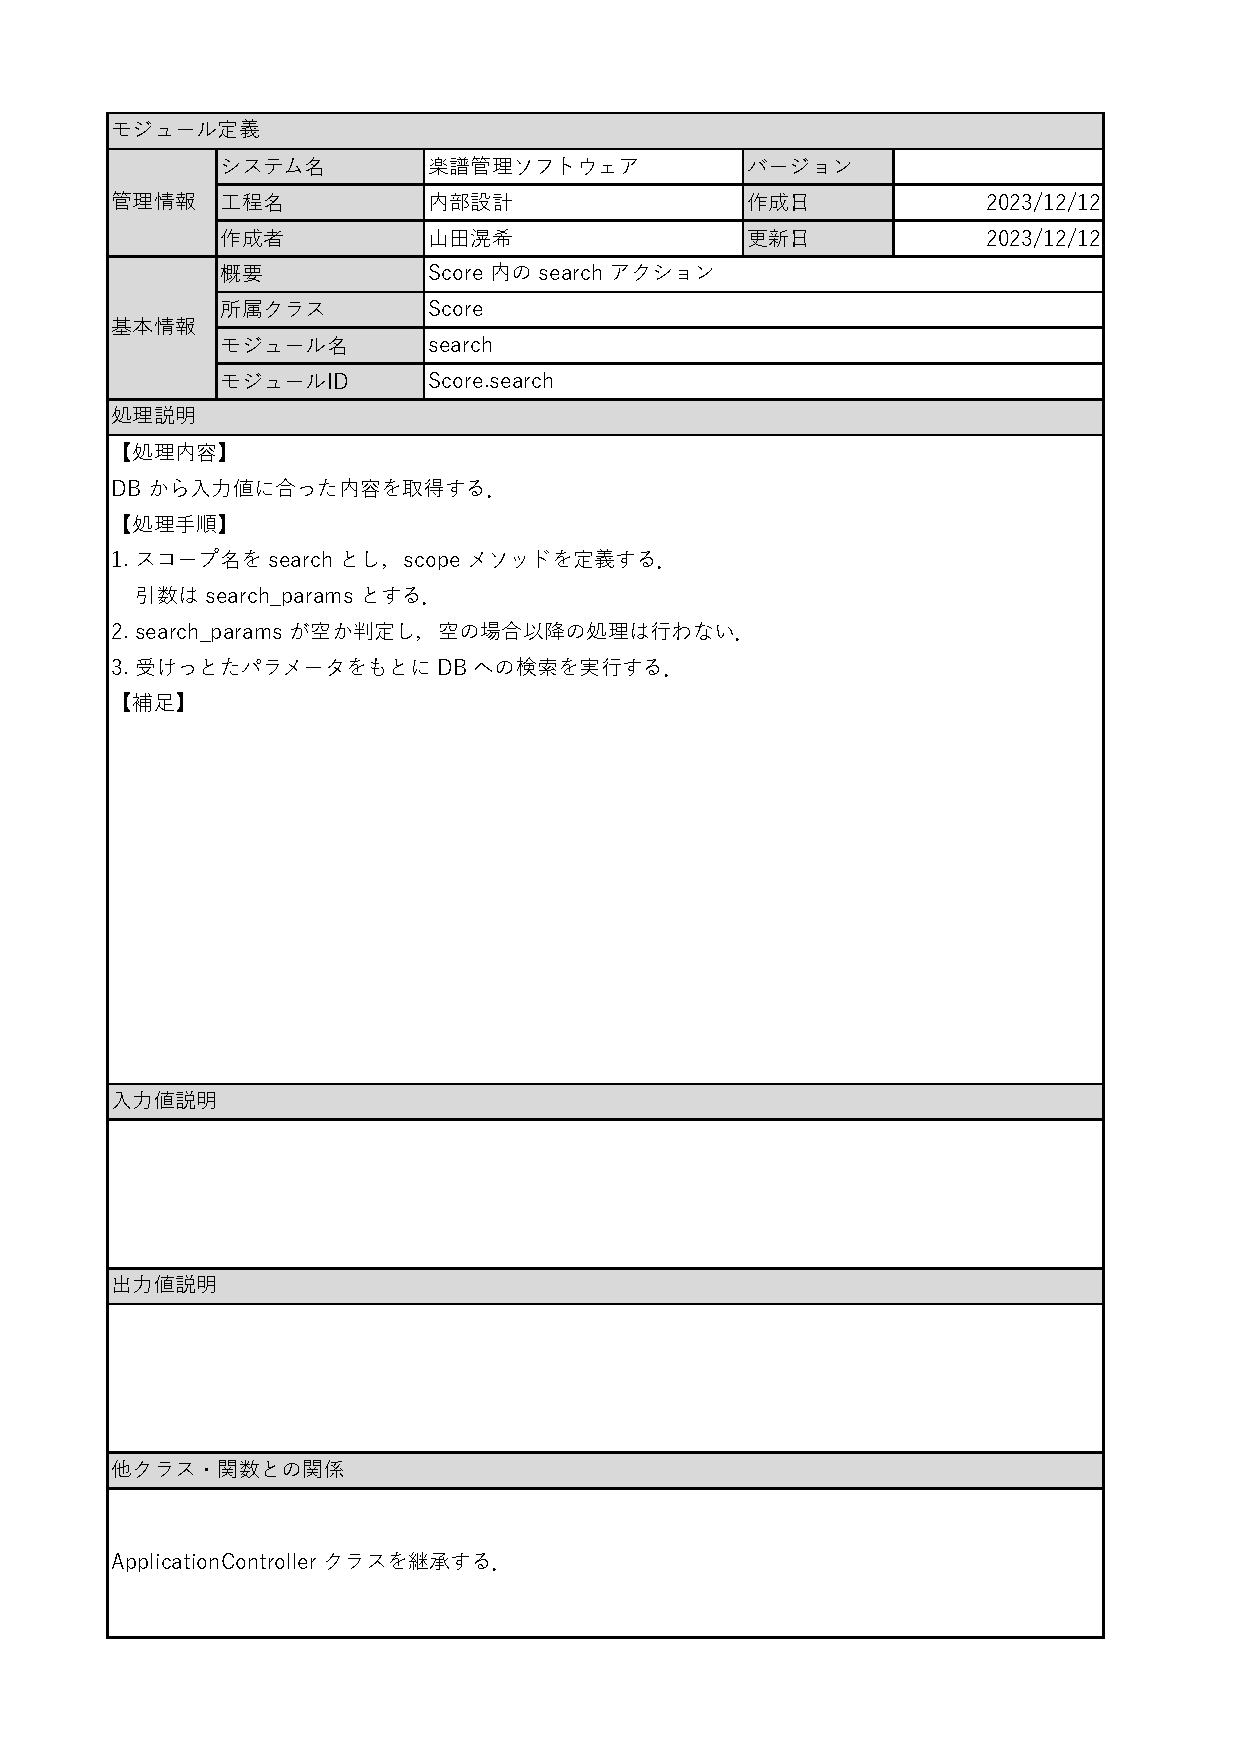
\includegraphics[scale=0.5]{img/Method/Score_search(scope).pdf}
    \caption{Score.score\_search}
\end{figure}
\clearpage

%使用楽器検索
\subsection*{楽譜を使用楽器から検索する機能}
チェックボックスへの入力を受け取り,マークされた楽器を含む楽譜を検索する機能.
\begin{figure}[H]
    \centering
    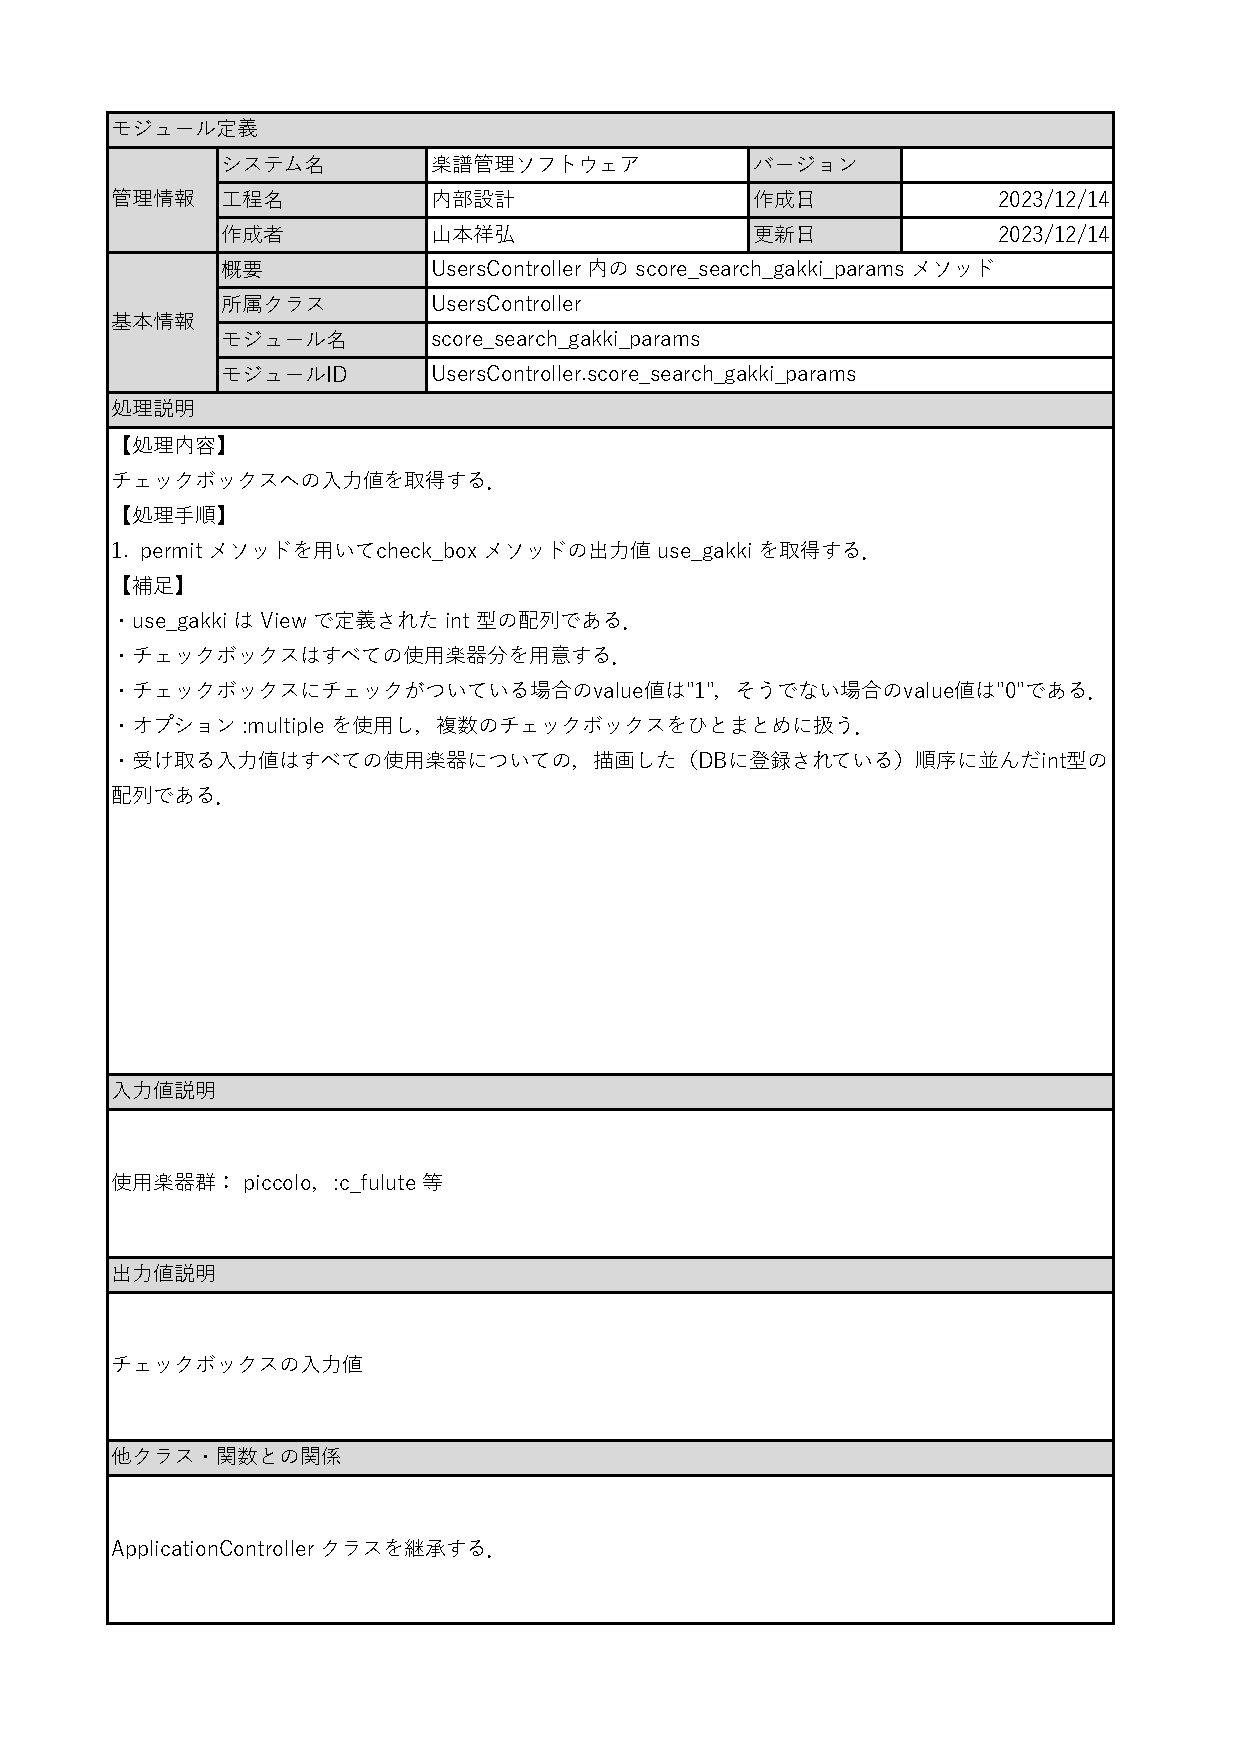
\includegraphics[scale=0.5]{img/Method/score_search_gakki_params.pdf}
    \caption{ScoresController.score\_search\_gakki\_params}
\end{figure}
\begin{figure}
    \centering
    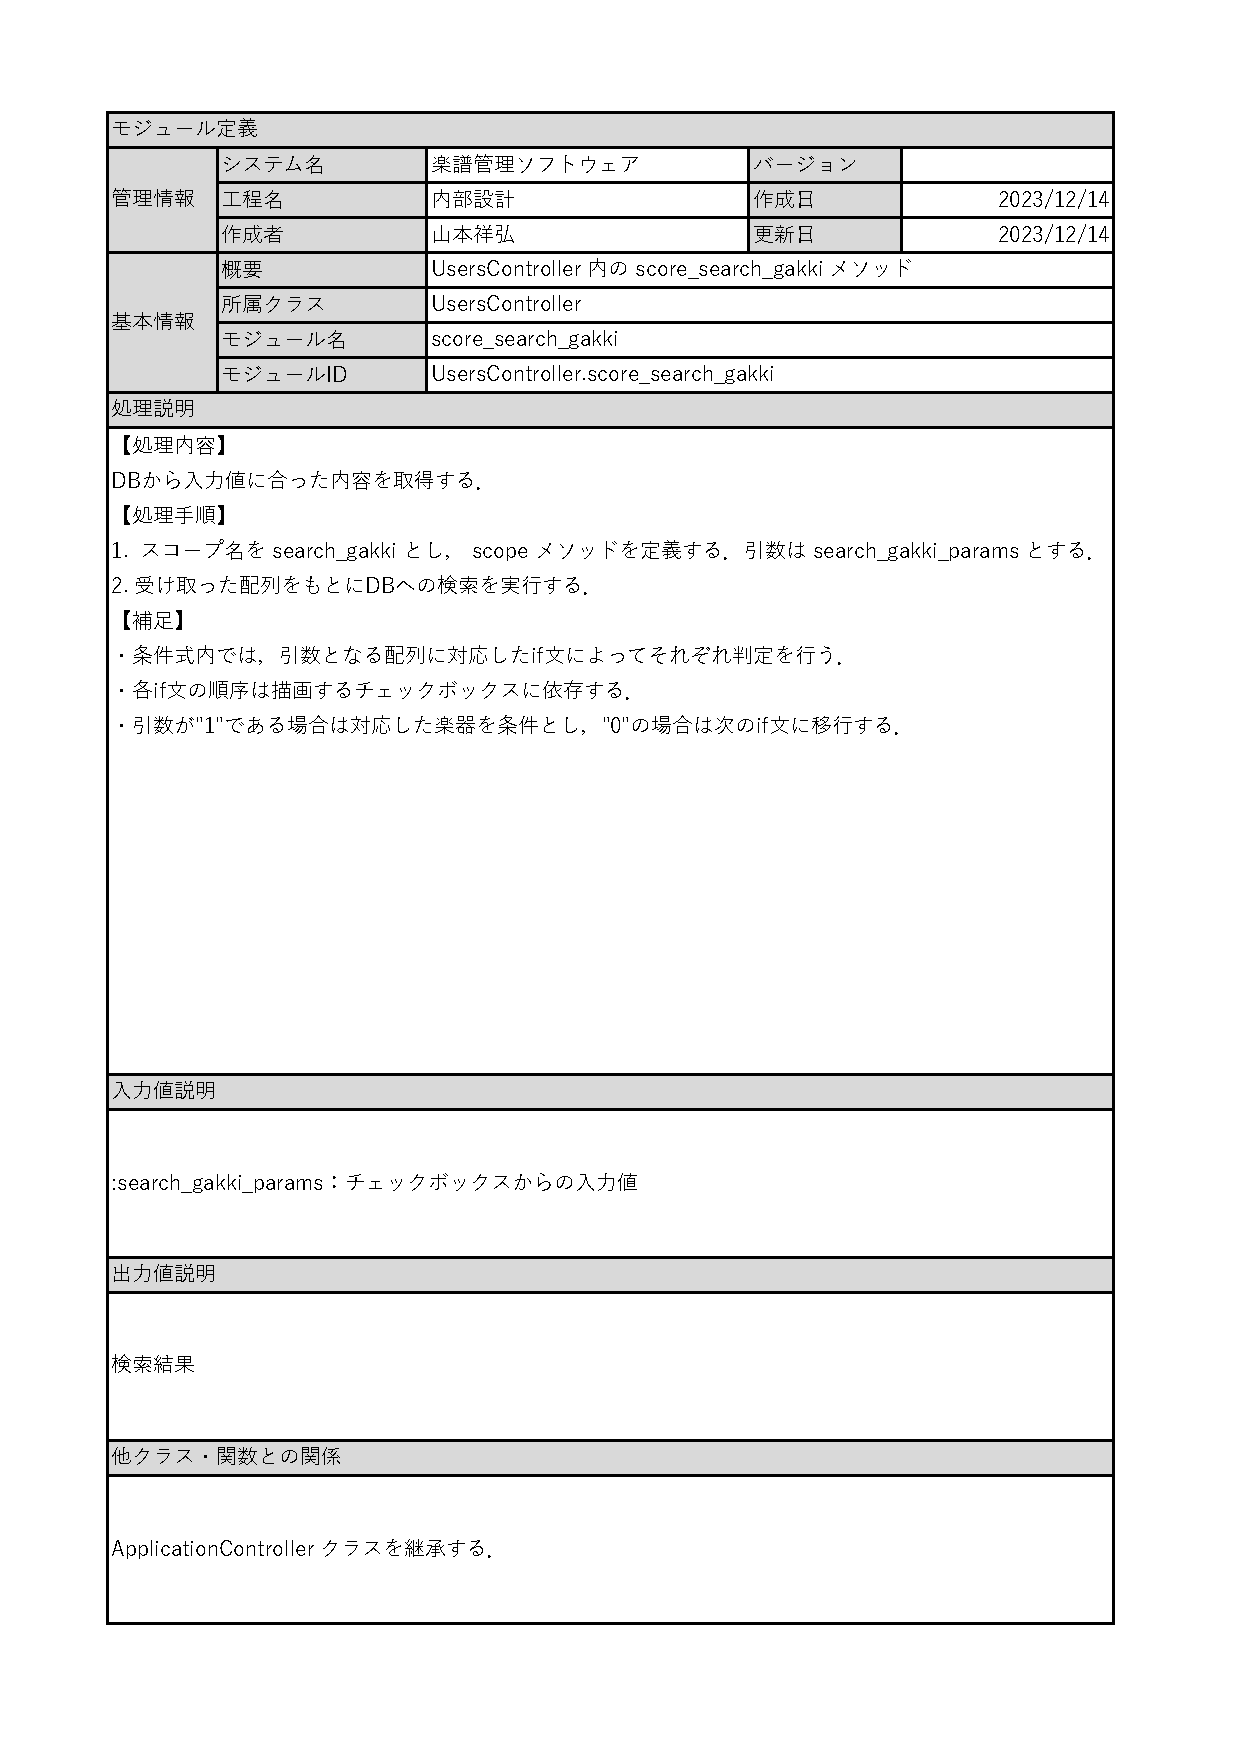
\includegraphics[scale=0.5]{img/Method/Scores_search_gakki(scope).pdf}
    \caption{Score.scores\_search\_gakki}
\end{figure}
\clearpage

%グレードソート
\subsection*{楽譜をグレードからソートする機能}
降順,昇順への並べ替えに使用される.また,図\ref{Score.grade-sort-no}は
データの作成順への並べ替えに使用される.
\begin{figure}[H]
    \centering
    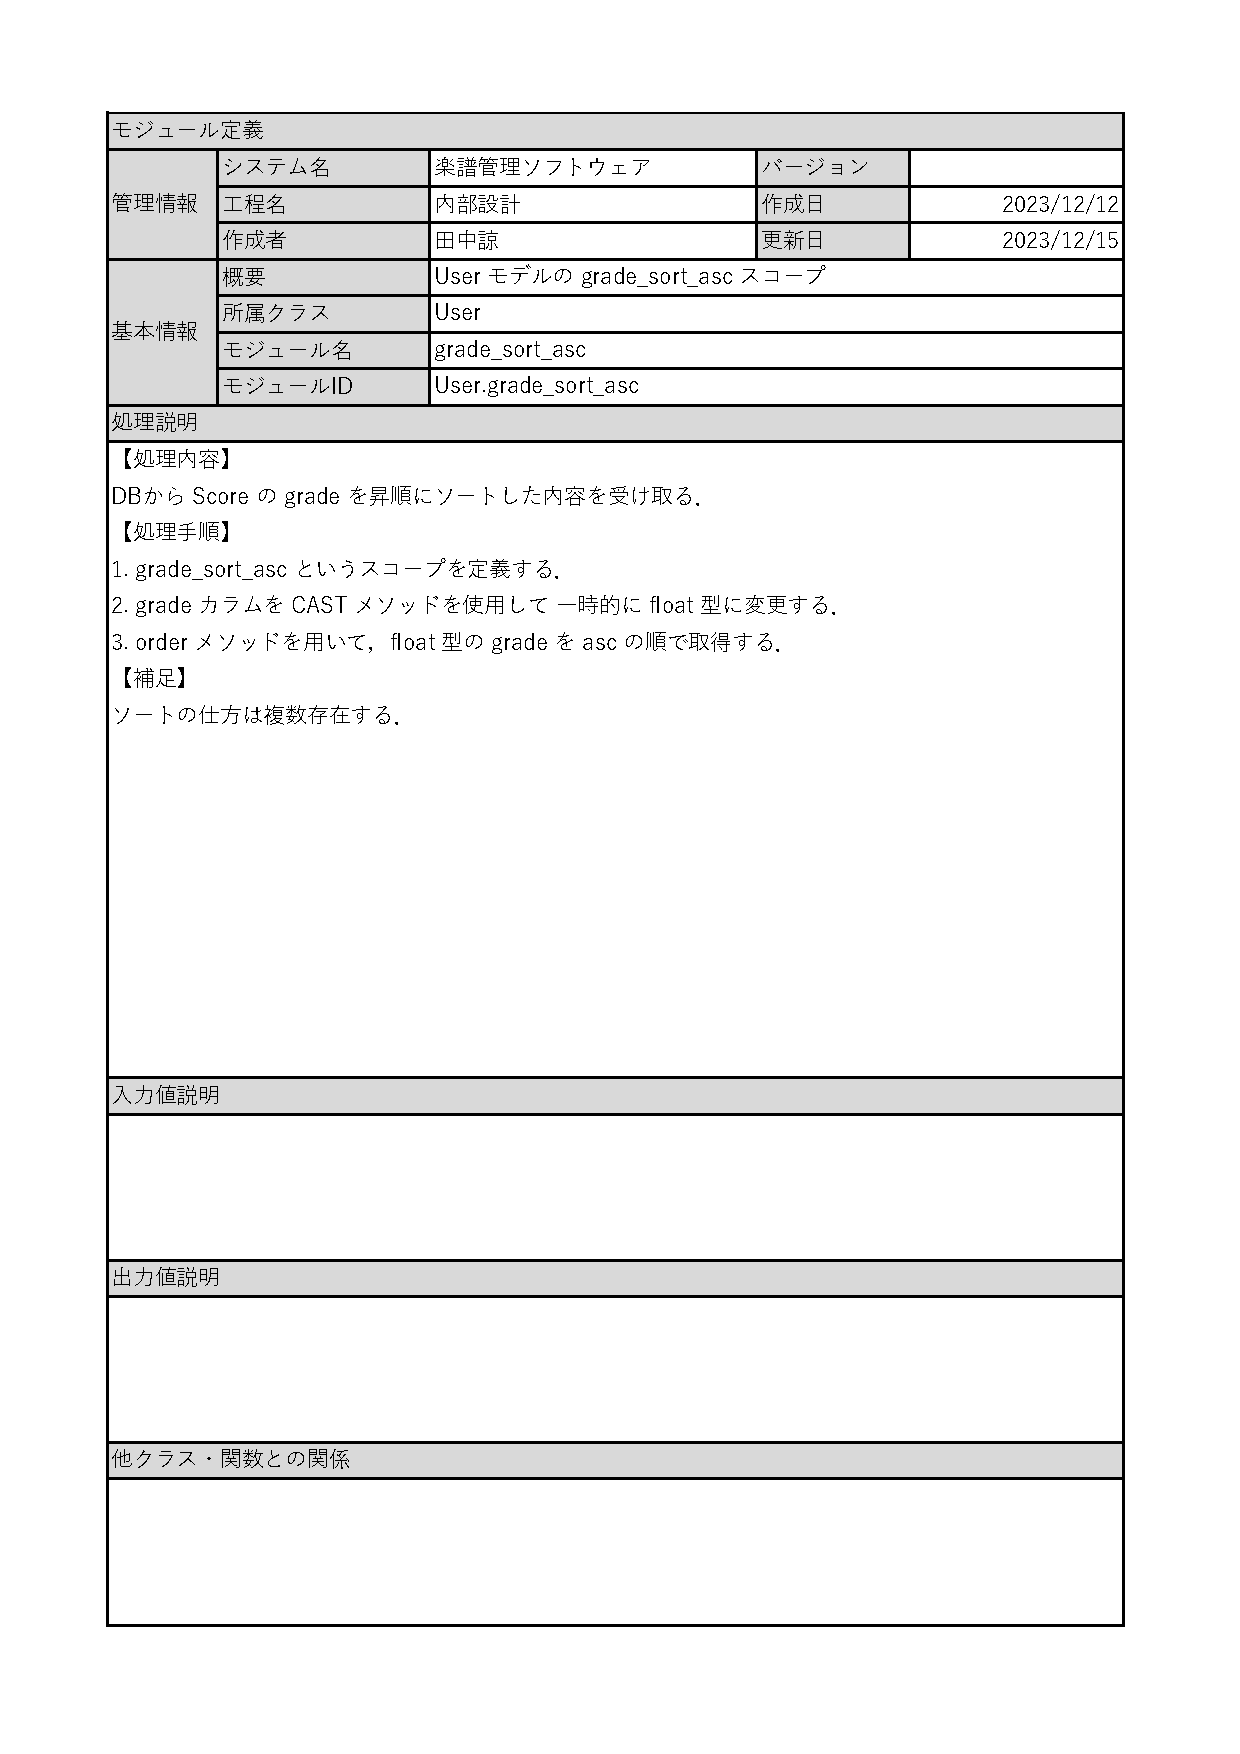
\includegraphics[scale=0.5]{img/Model/gradeSort_asc.pdf}
    \caption{Score.grade\_sort\_asc}
\end{figure}
\begin{figure}
    \centering
    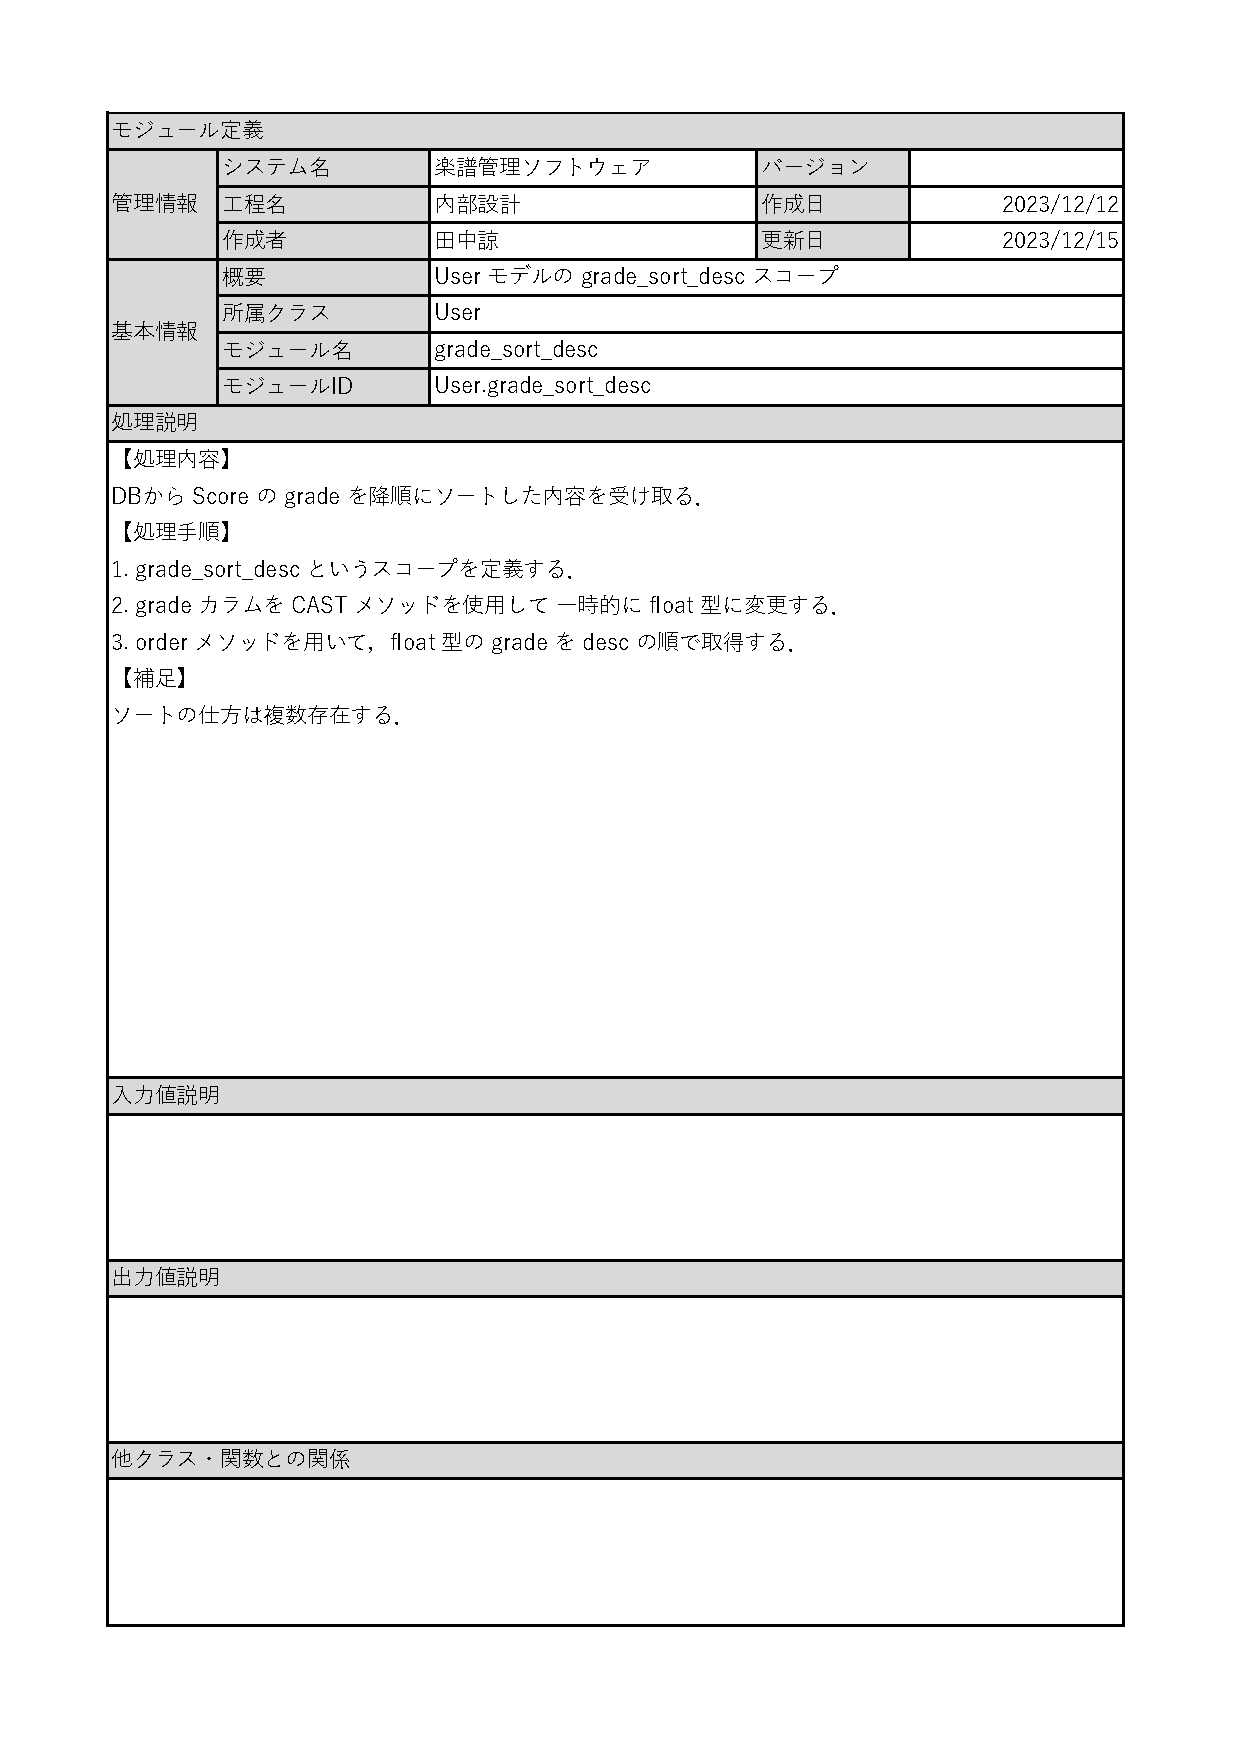
\includegraphics[scale=0.5]{img/Model/gradeSort_desc.pdf}
    \caption{Score.grade\_sort\_desc}
\end{figure}
\begin{figure}
    \centering
    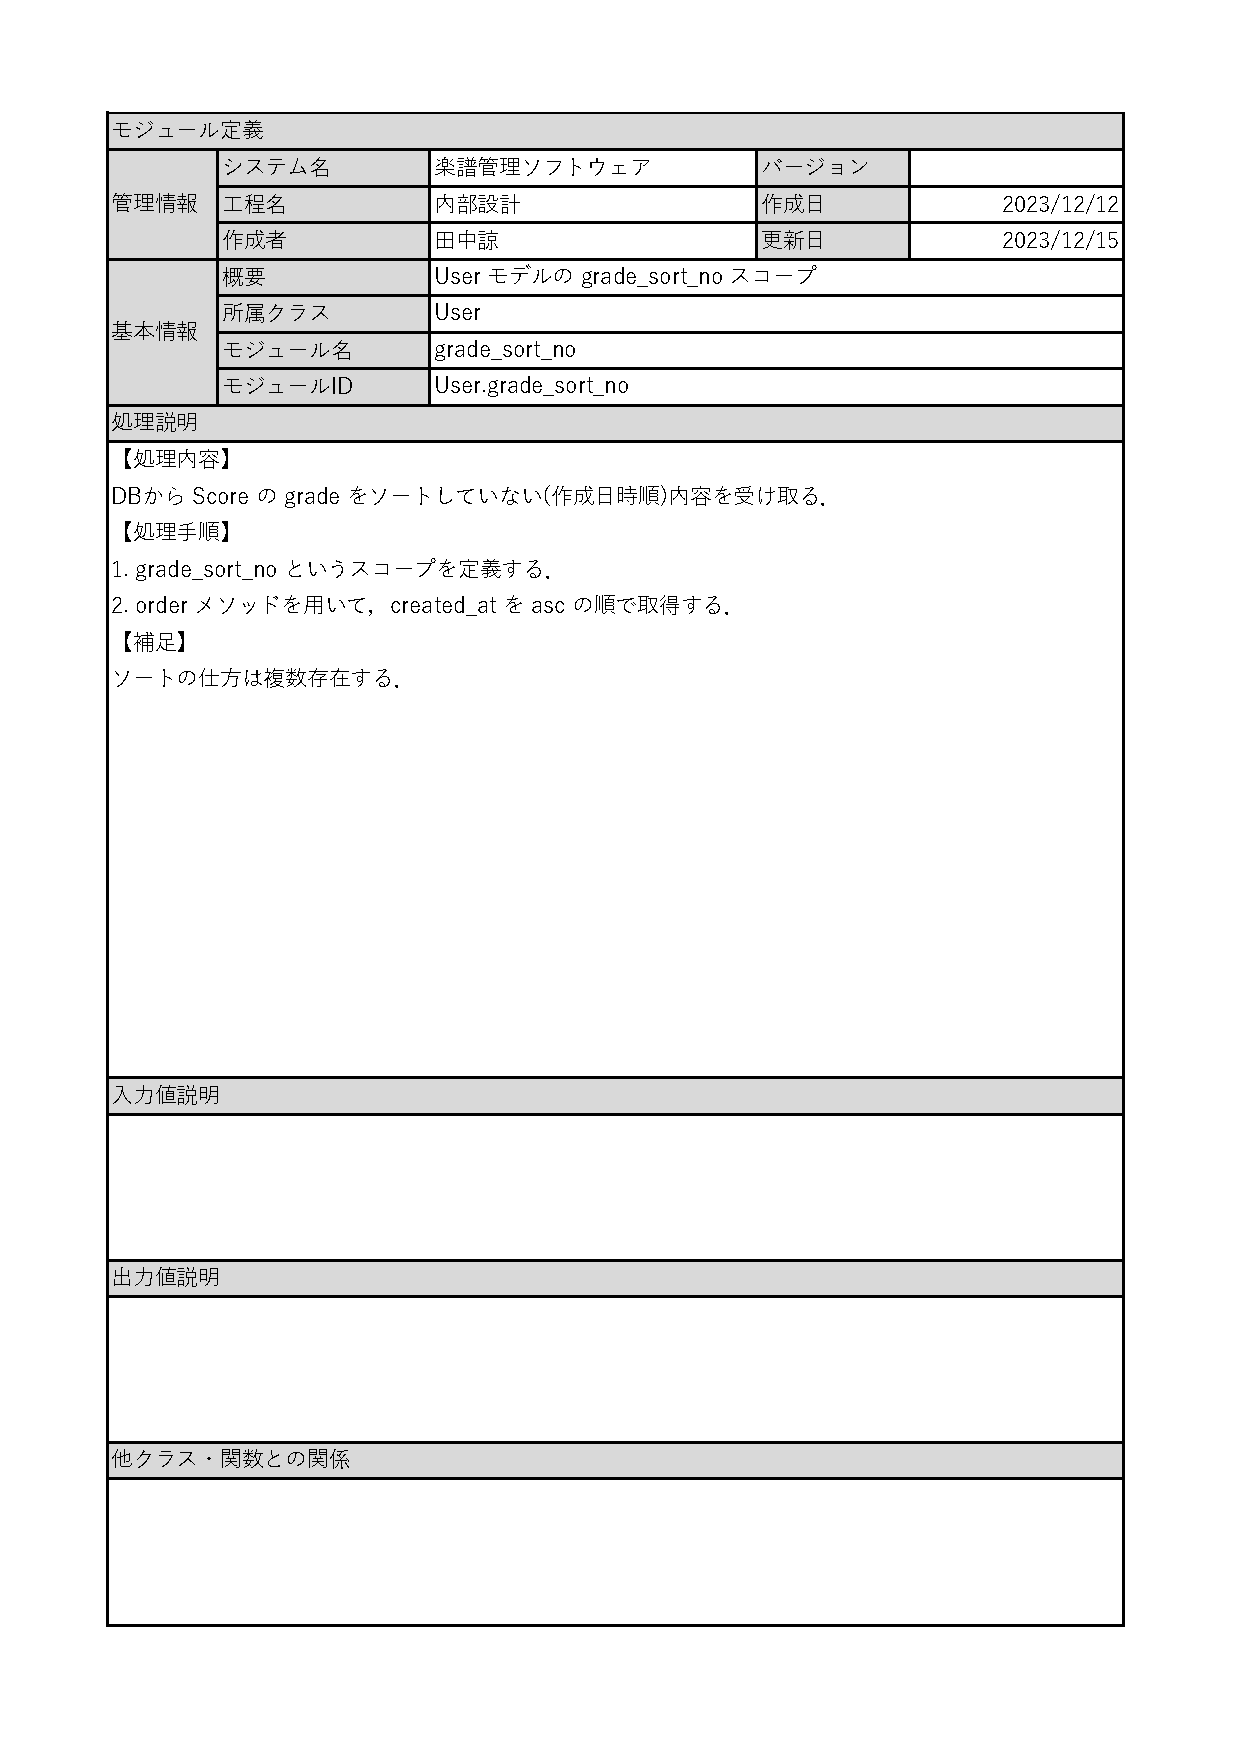
\includegraphics[scale=0.5]{img/Model/gradeSort_no.pdf}
    \caption{Score.grade\_sort\_no}
    \label{Score.grade-sort-no}
\end{figure}
\clearpage

%ユーザ検索
\subsection*{ユーザをユーザ名・ユーザIDから検索する機能}
検索ボックスへの入力値を受け取り,入力文字列を含むデータを検索する機能.
\begin{figure}[H]
    \centering
    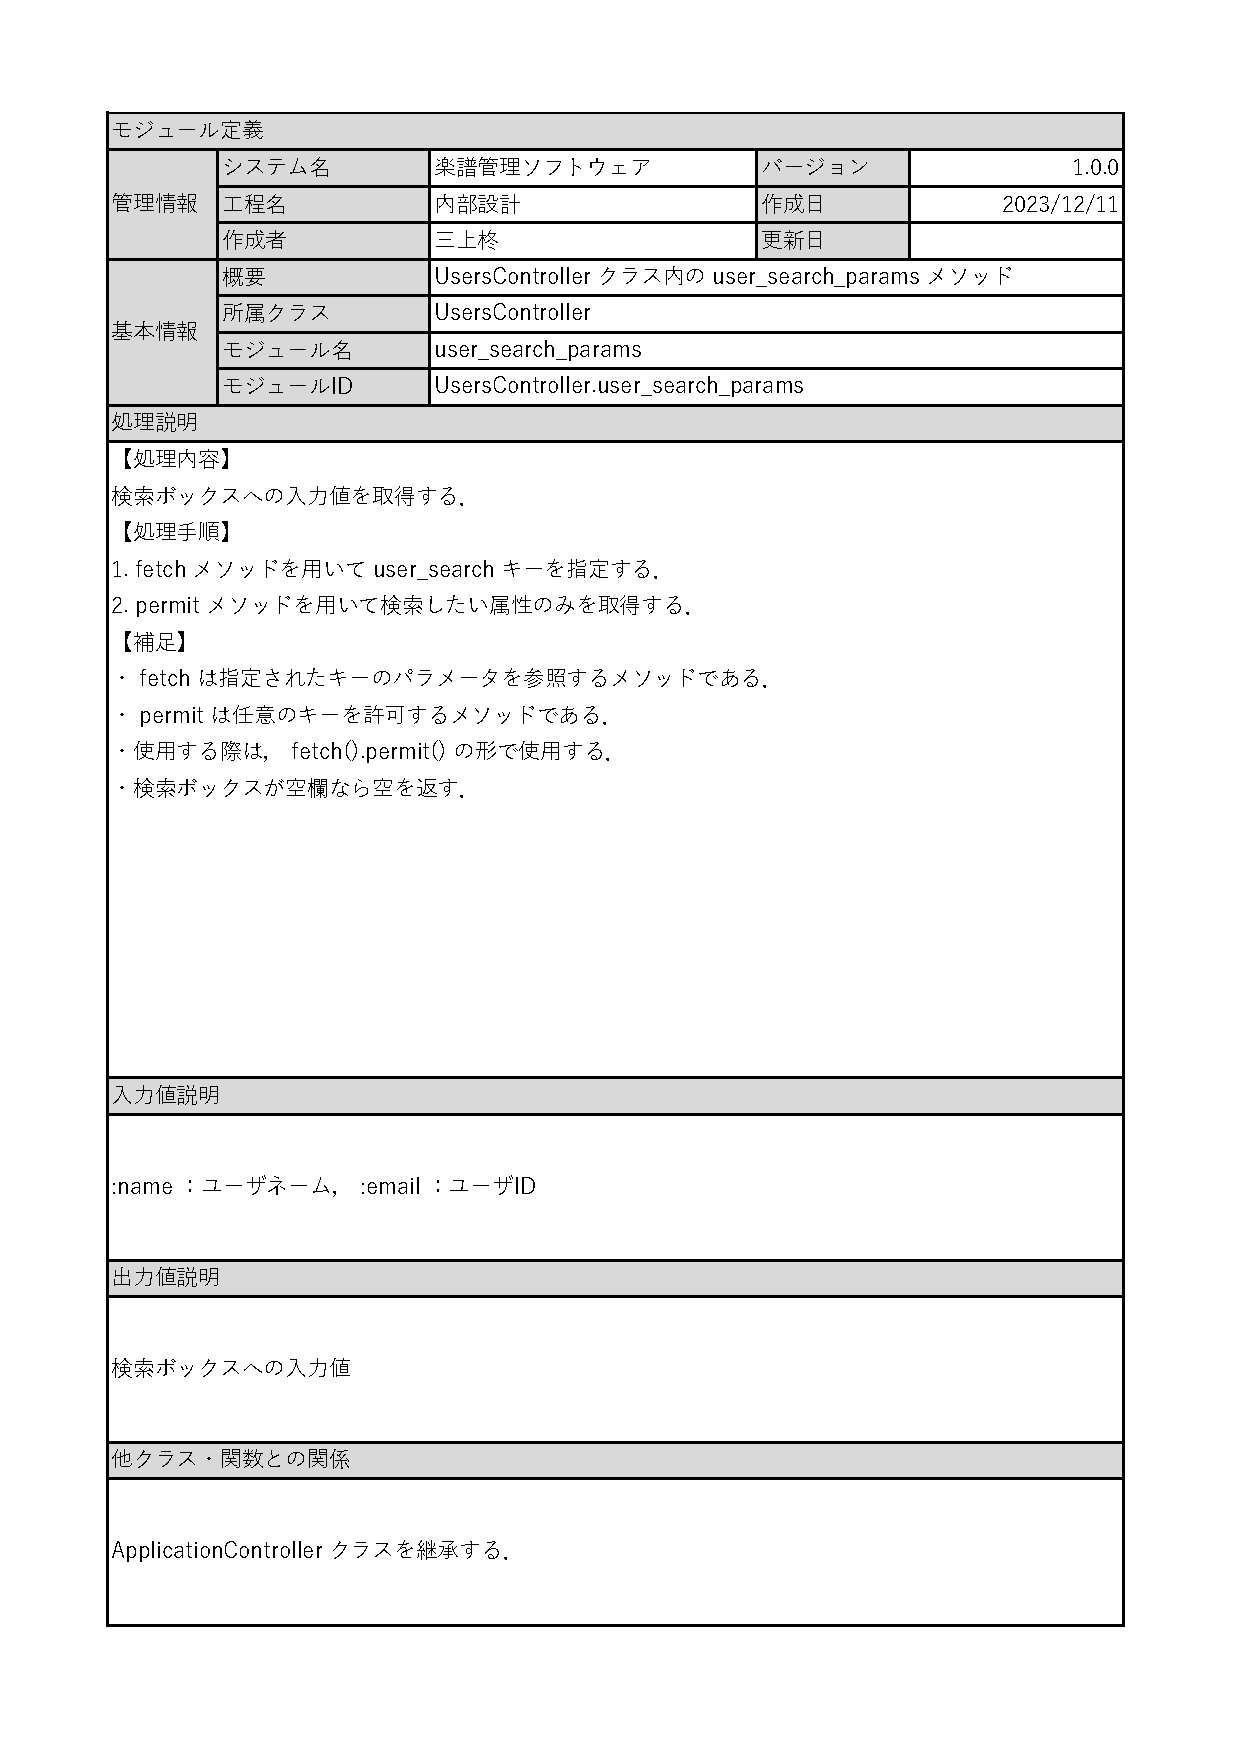
\includegraphics[scale=0.5]{img/Method/user_search_params.pdf}
    \caption{UsersController.user\_search\_params}
\end{figure}
\begin{figure}
    \centering
    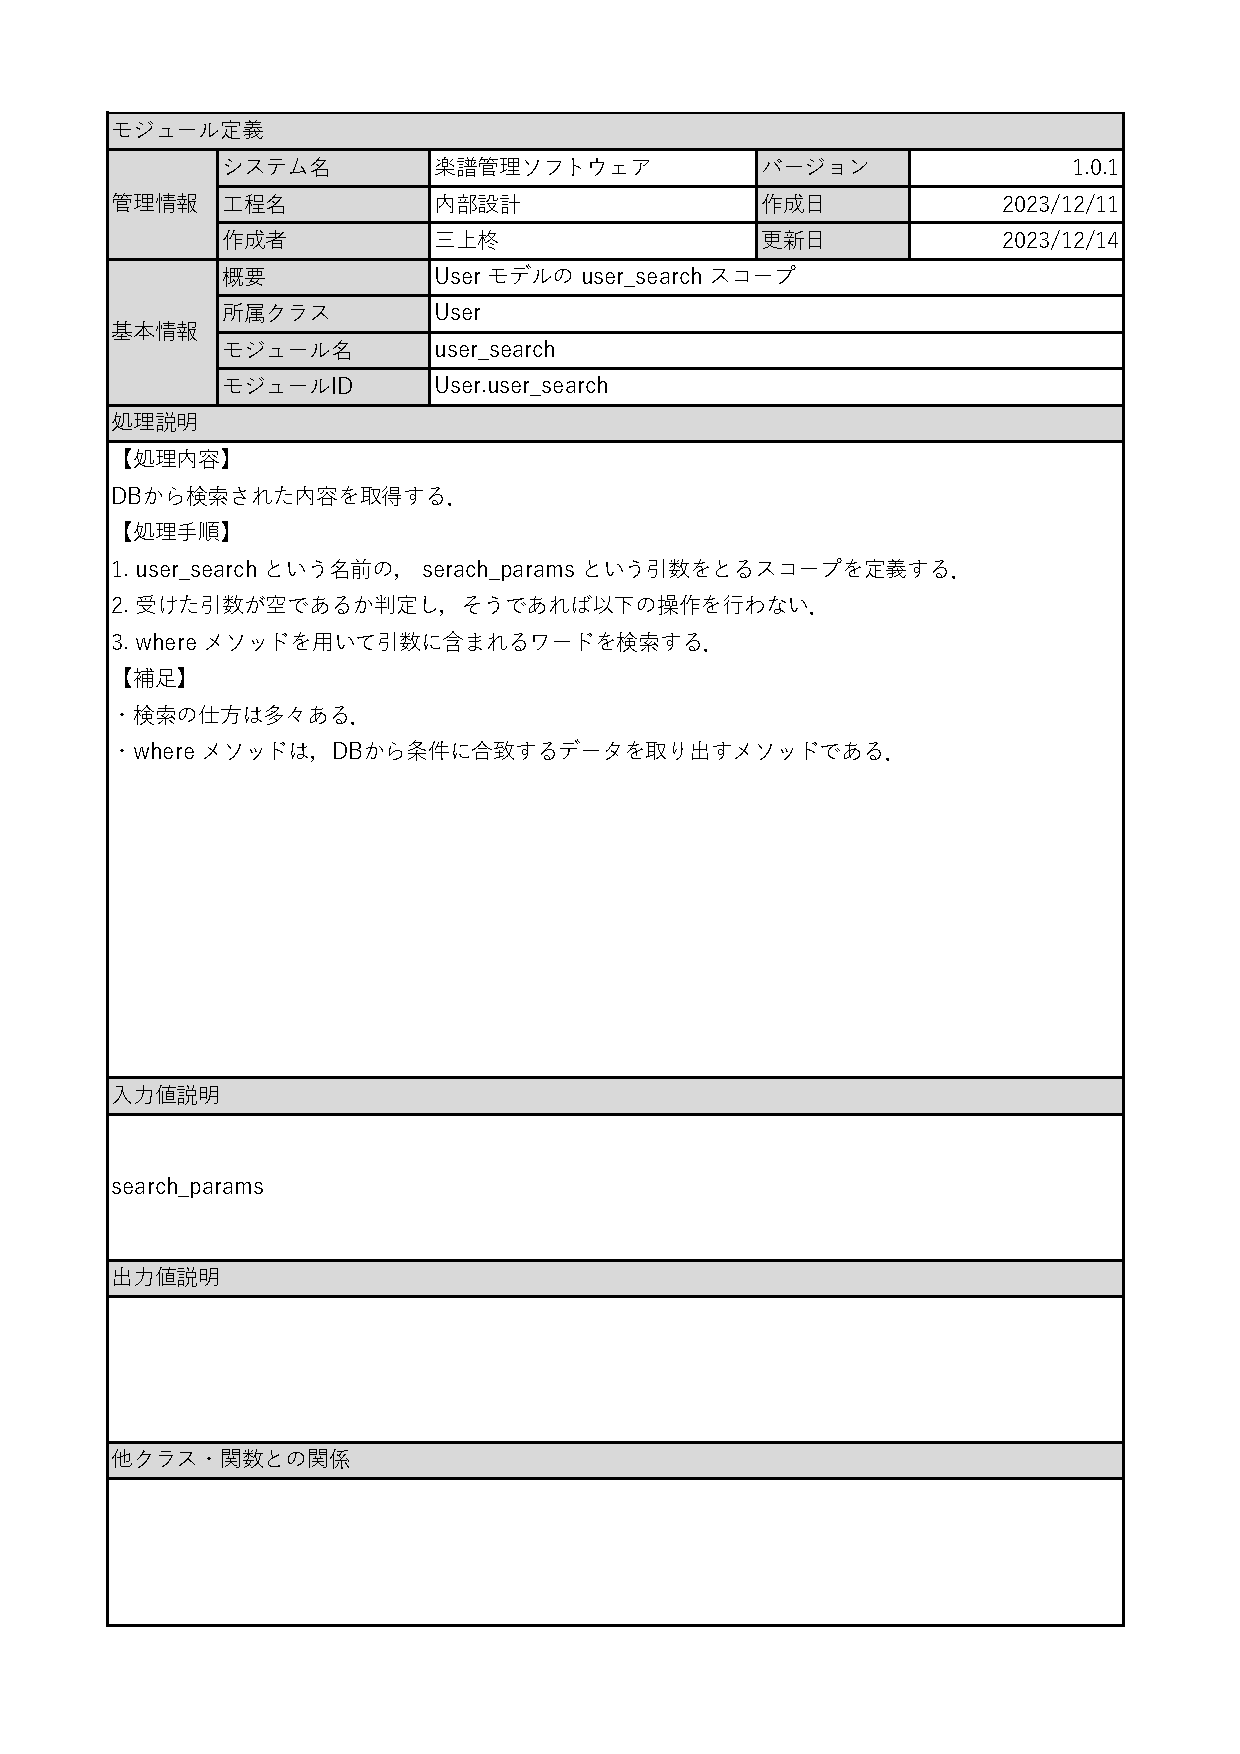
\includegraphics[scale=0.5]{img/Method/User_search(scope).pdf}
    \caption{User.user\_search}
\end{figure}
\clearpage

%ログイン処理
\subsection*{ログイン処理機能}
ユーザのログイン処理を行う機能.
\begin{figure}[H]
    \centering
    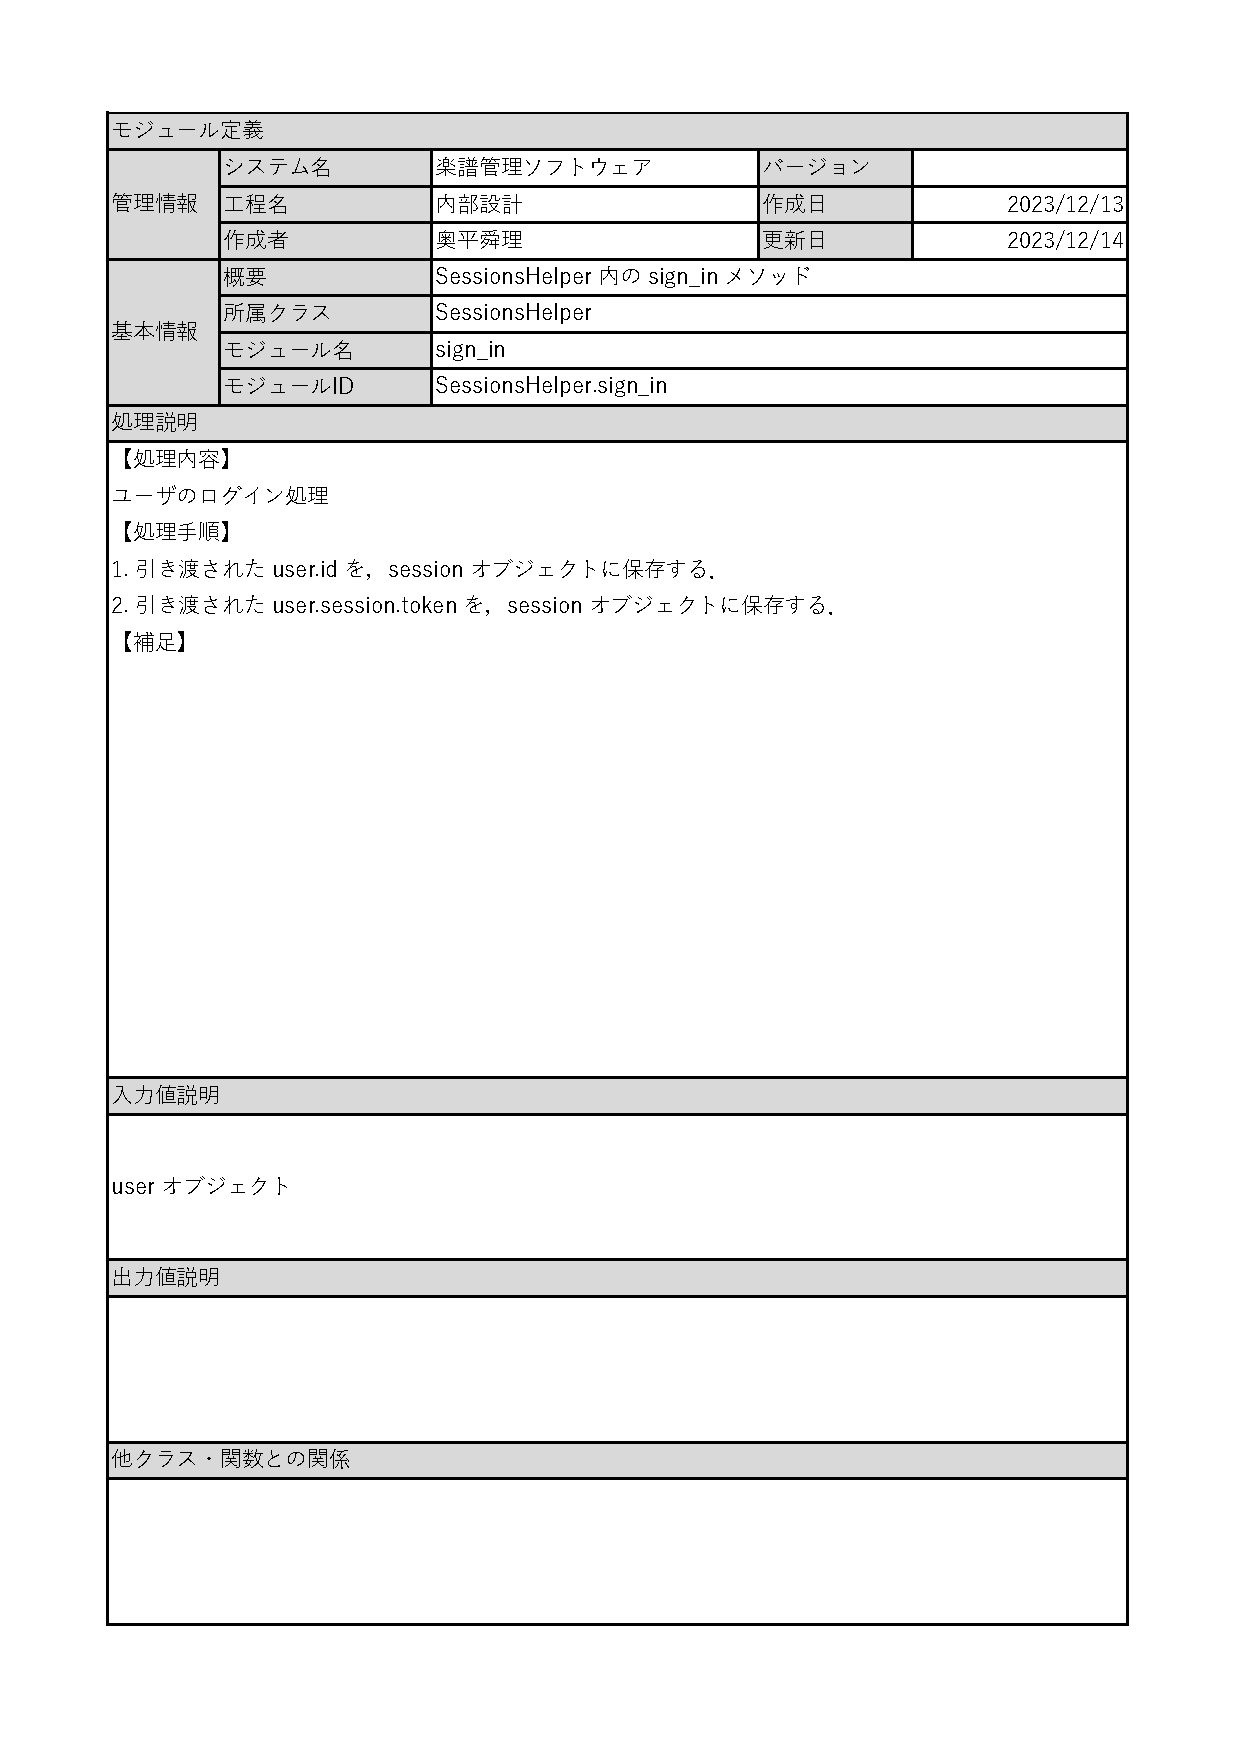
\includegraphics[scale=0.5]{img/Helper/sign_in.pdf}
    \caption{SessionsHelper.sign\_in}
\end{figure}
\clearpage

%ログイン判定
\subsection*{ユーザがログイン中か判定する機能}
意図しない方法でのアクセスを無視するために使用される.
\begin{figure}[H]
    \centering
    \includegraphics[scale=0.5]{img/Helper/sign_in?.pdf}
    \caption{SessionsHelper.sign\_in?}
    \label{SessionsHelper.sign-in?}
\end{figure}
\clearpage

%不正防止
\subsection*{ユーザがログイン中でない場合にログインページへリダイレクトする機能}
意図しない方法でアクセスされた場合にログインページへ遷移するために使用される.
\begin{figure}[H]
    \centering
    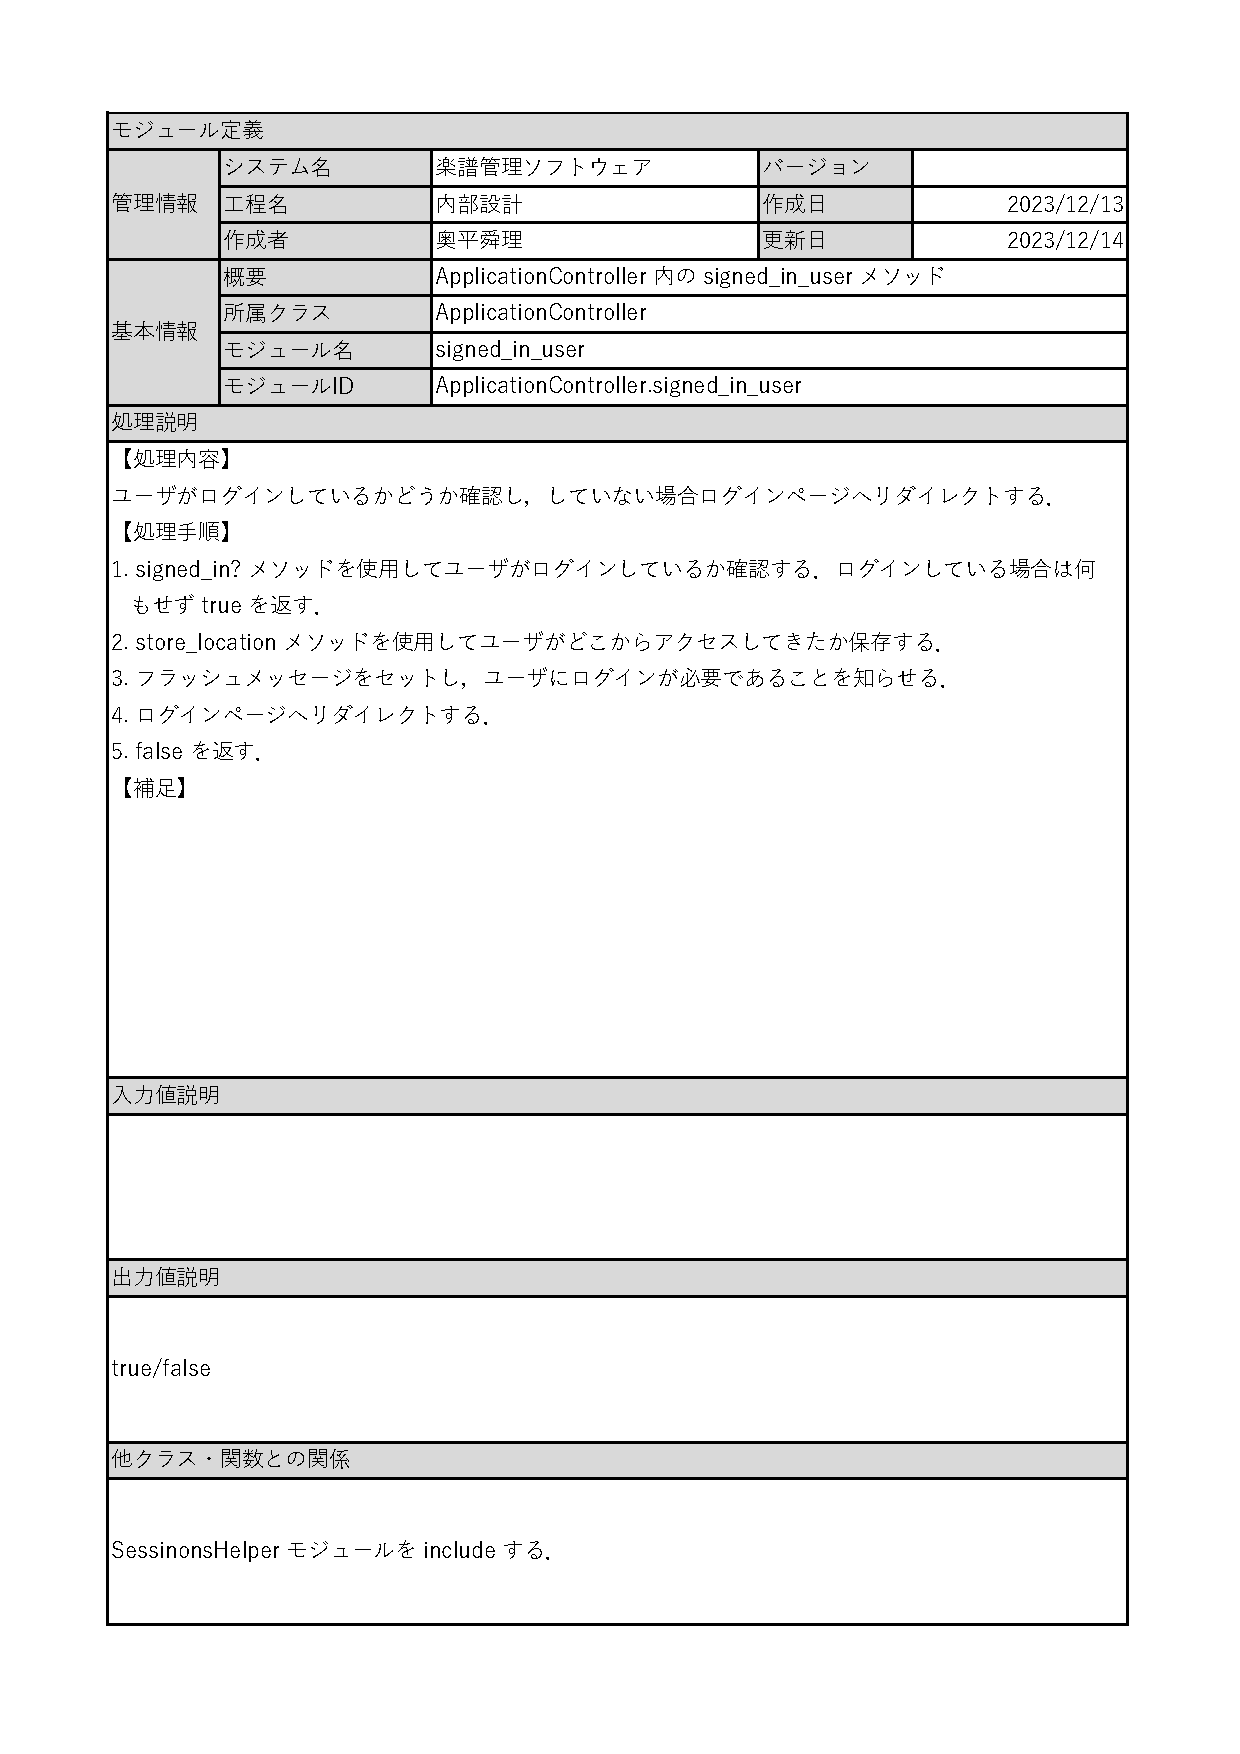
\includegraphics[scale=0.5]{img/Helper/signed_in_user.pdf}
    \caption{SessionsHelper.signed\/in\_user}
\end{figure}
\clearpage

%Cookie保存
\subsection*{ユーザの保持機能}
ユーザのCookie情報の保存に使用される.
\begin{figure}[H]
    \centering
    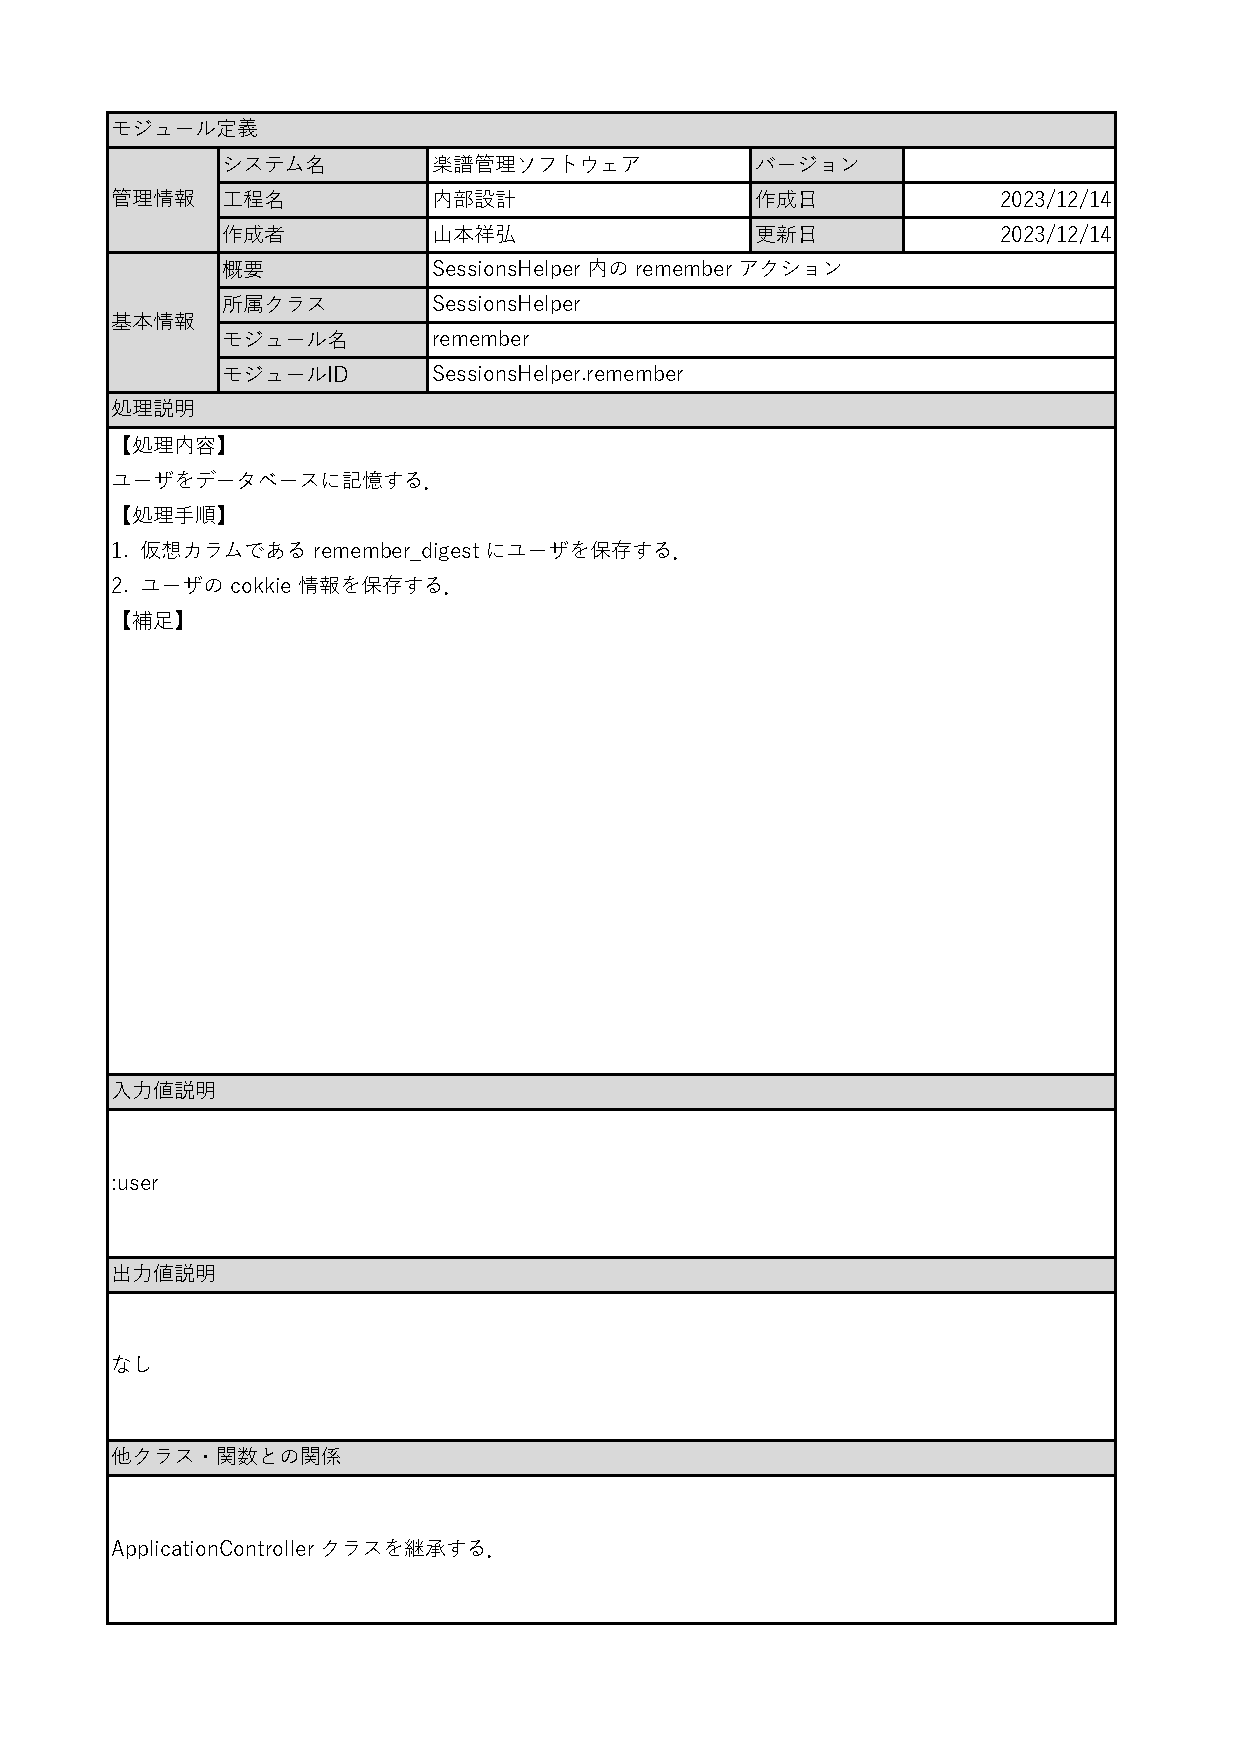
\includegraphics[scale=0.5]{img/Helper/SessionsHelper.remember.pdf}
    \caption{SessionsHelper.remember}
\end{figure}
\clearpage

%ユーザ識別
\subsection*{現在のユーザを識別する機能}
題の通り.
\begin{figure}[H]
    \centering
    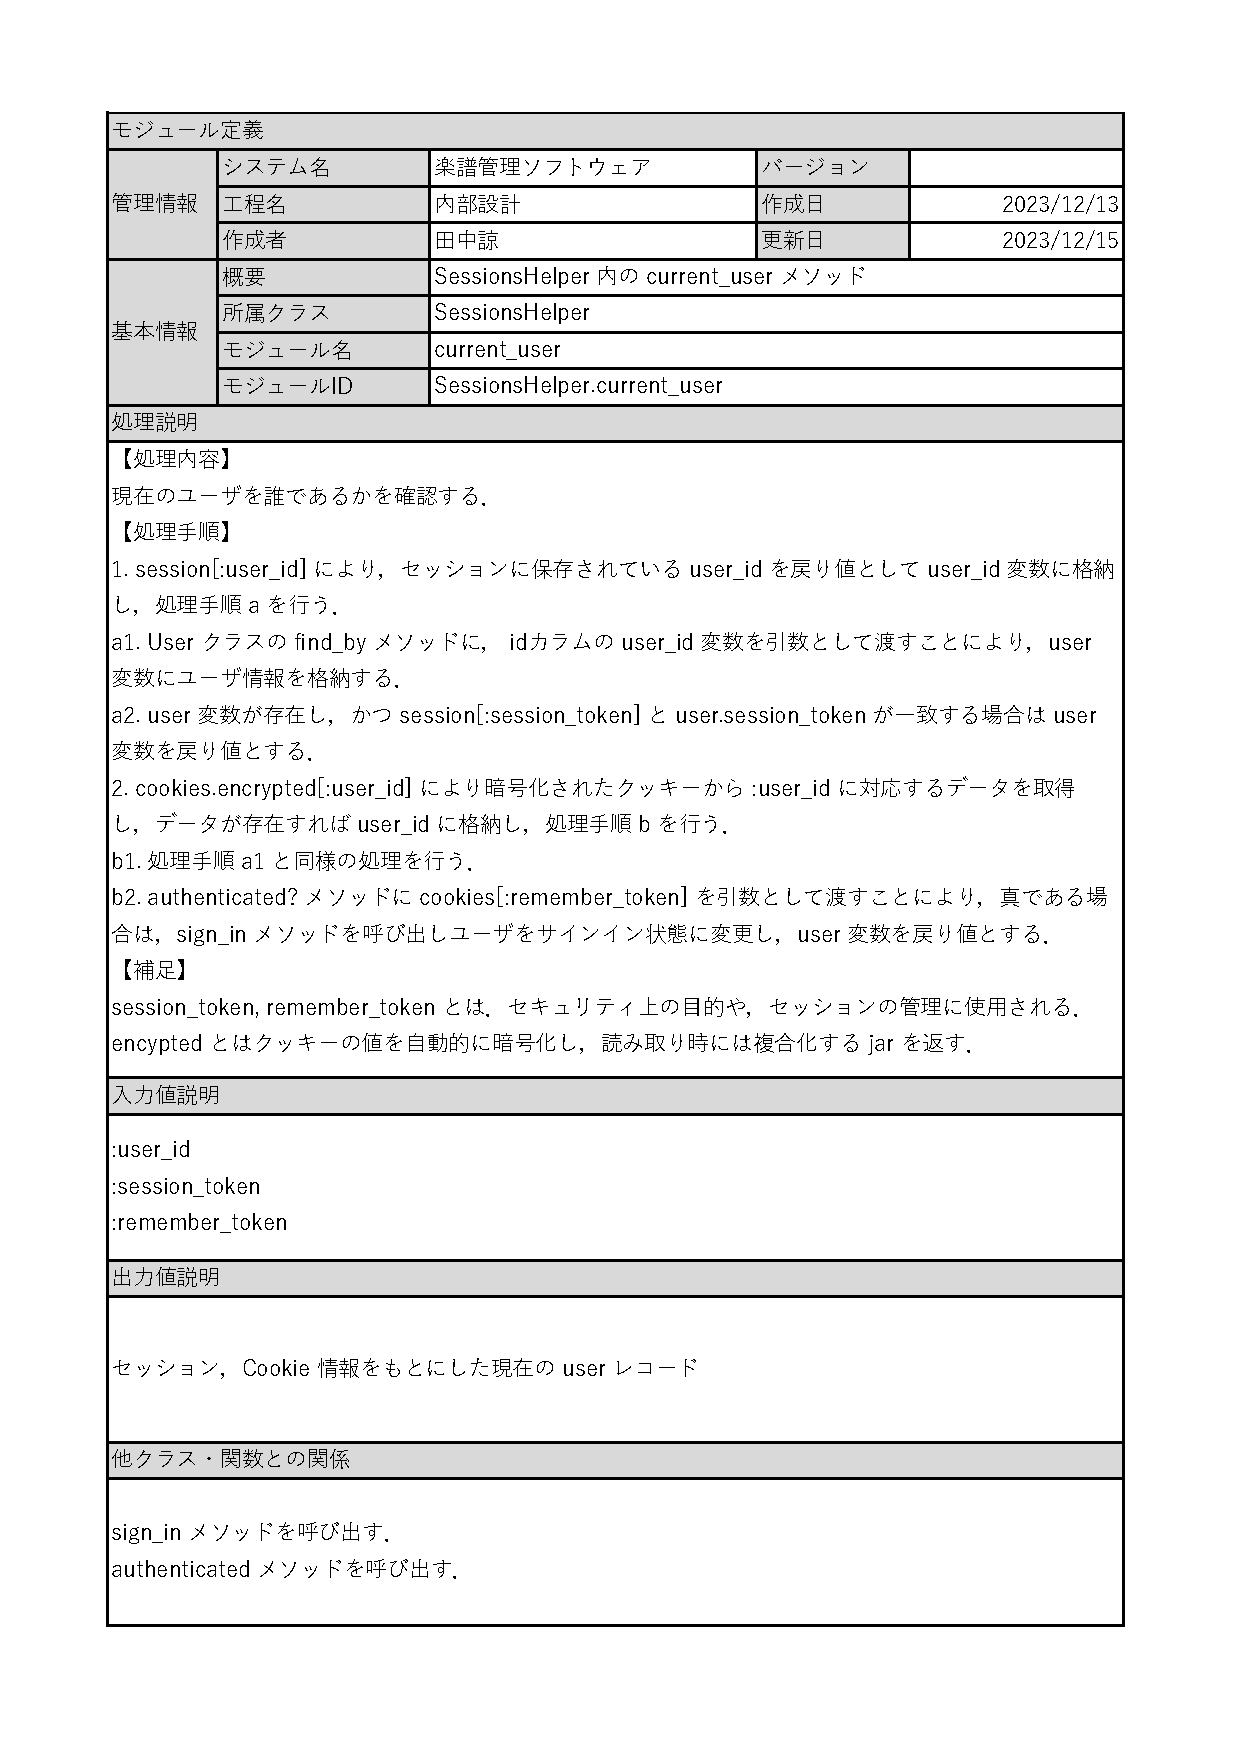
\includegraphics[scale=0.5]{img/Helper/current_user.pdf}
    \caption{SessionsHelper.current\_user}
\end{figure}
\clearpage

%ユーザ判定
\subsection*{渡されたユーザが現在ログインしているユーザか判定する機能.}
題の通り.
\begin{figure}[H]
    \centering
    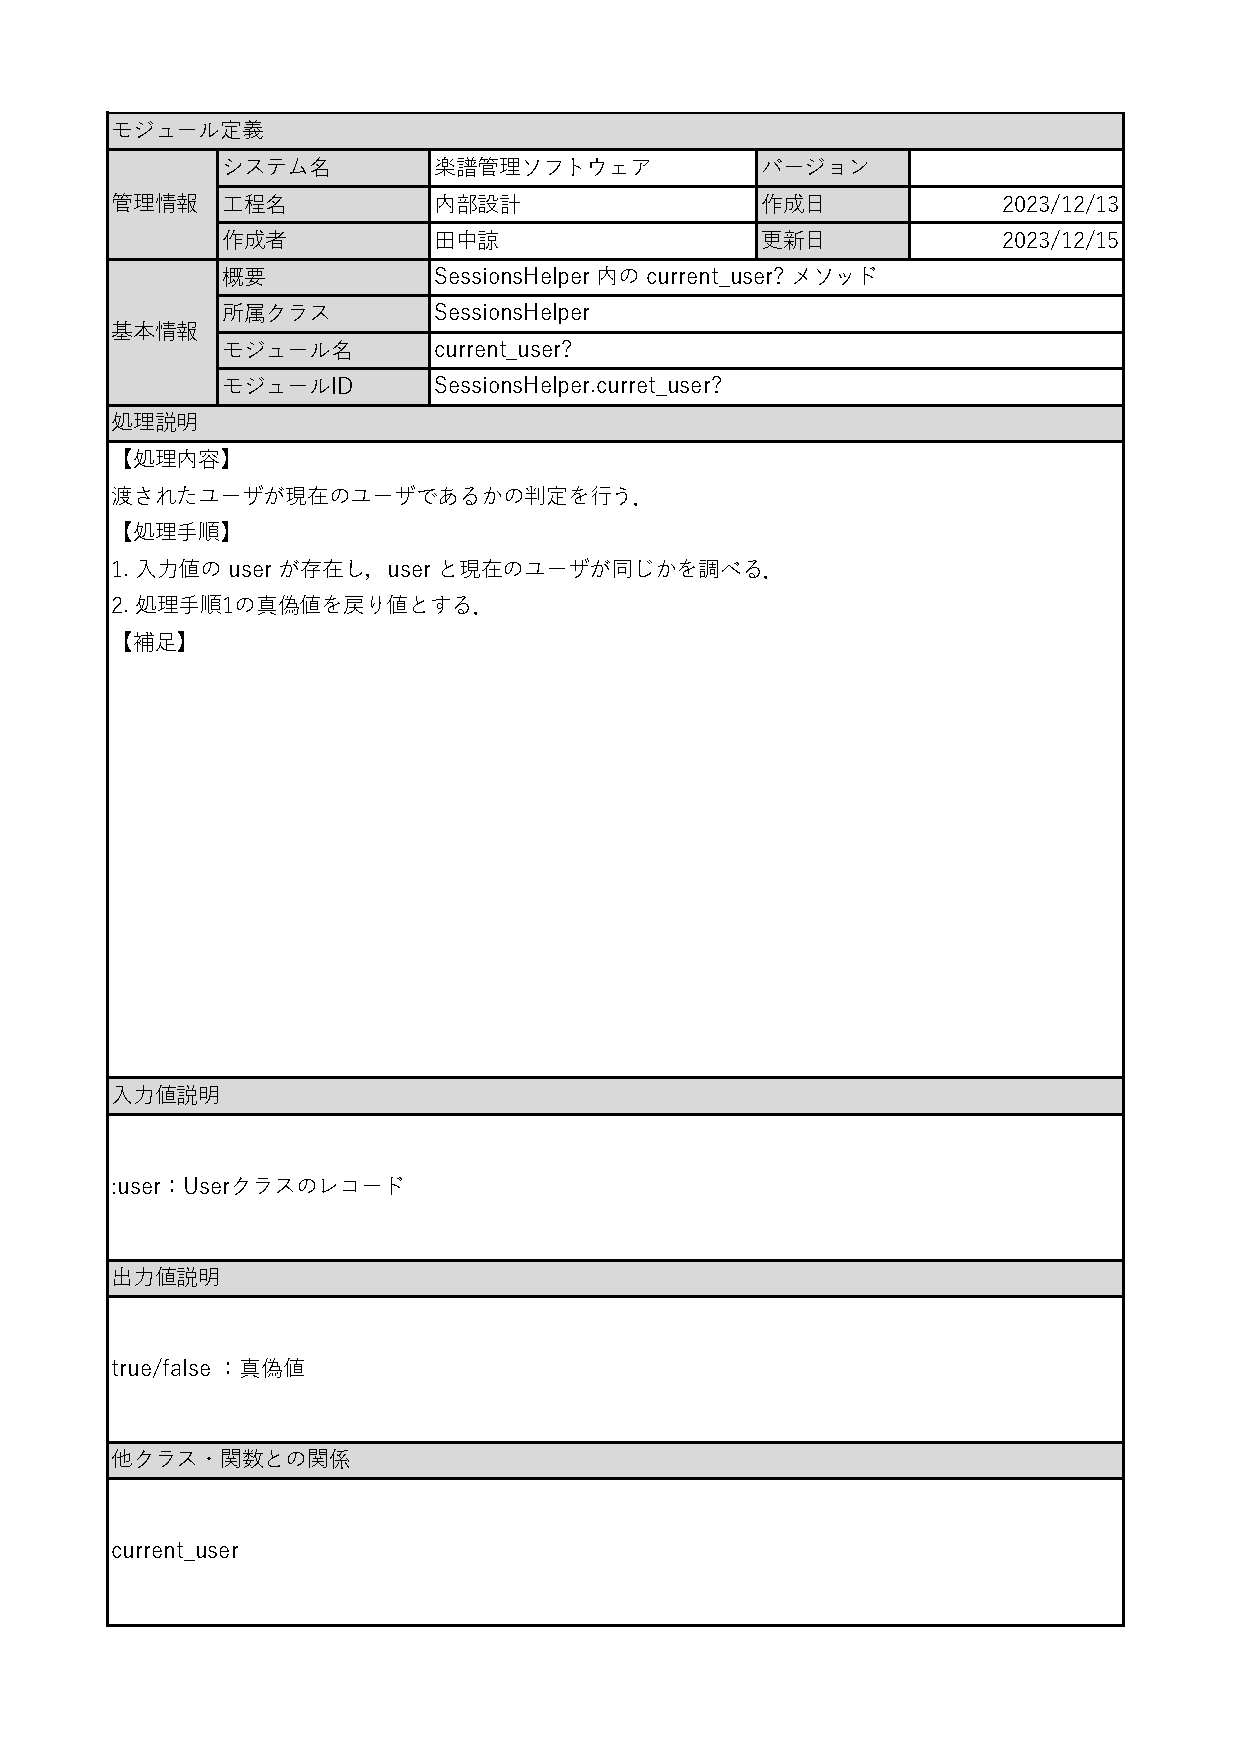
\includegraphics[scale=0.5]{img/Helper/current_user_boolean.pdf}
    \caption{SessionsHelper.current\_user?}
\end{figure}
\clearpage

%Cookie削除
\subsection*{Cookie情報を削除する機能}
ログアウト処理で使用される.
\begin{figure}[H]
    \centering
    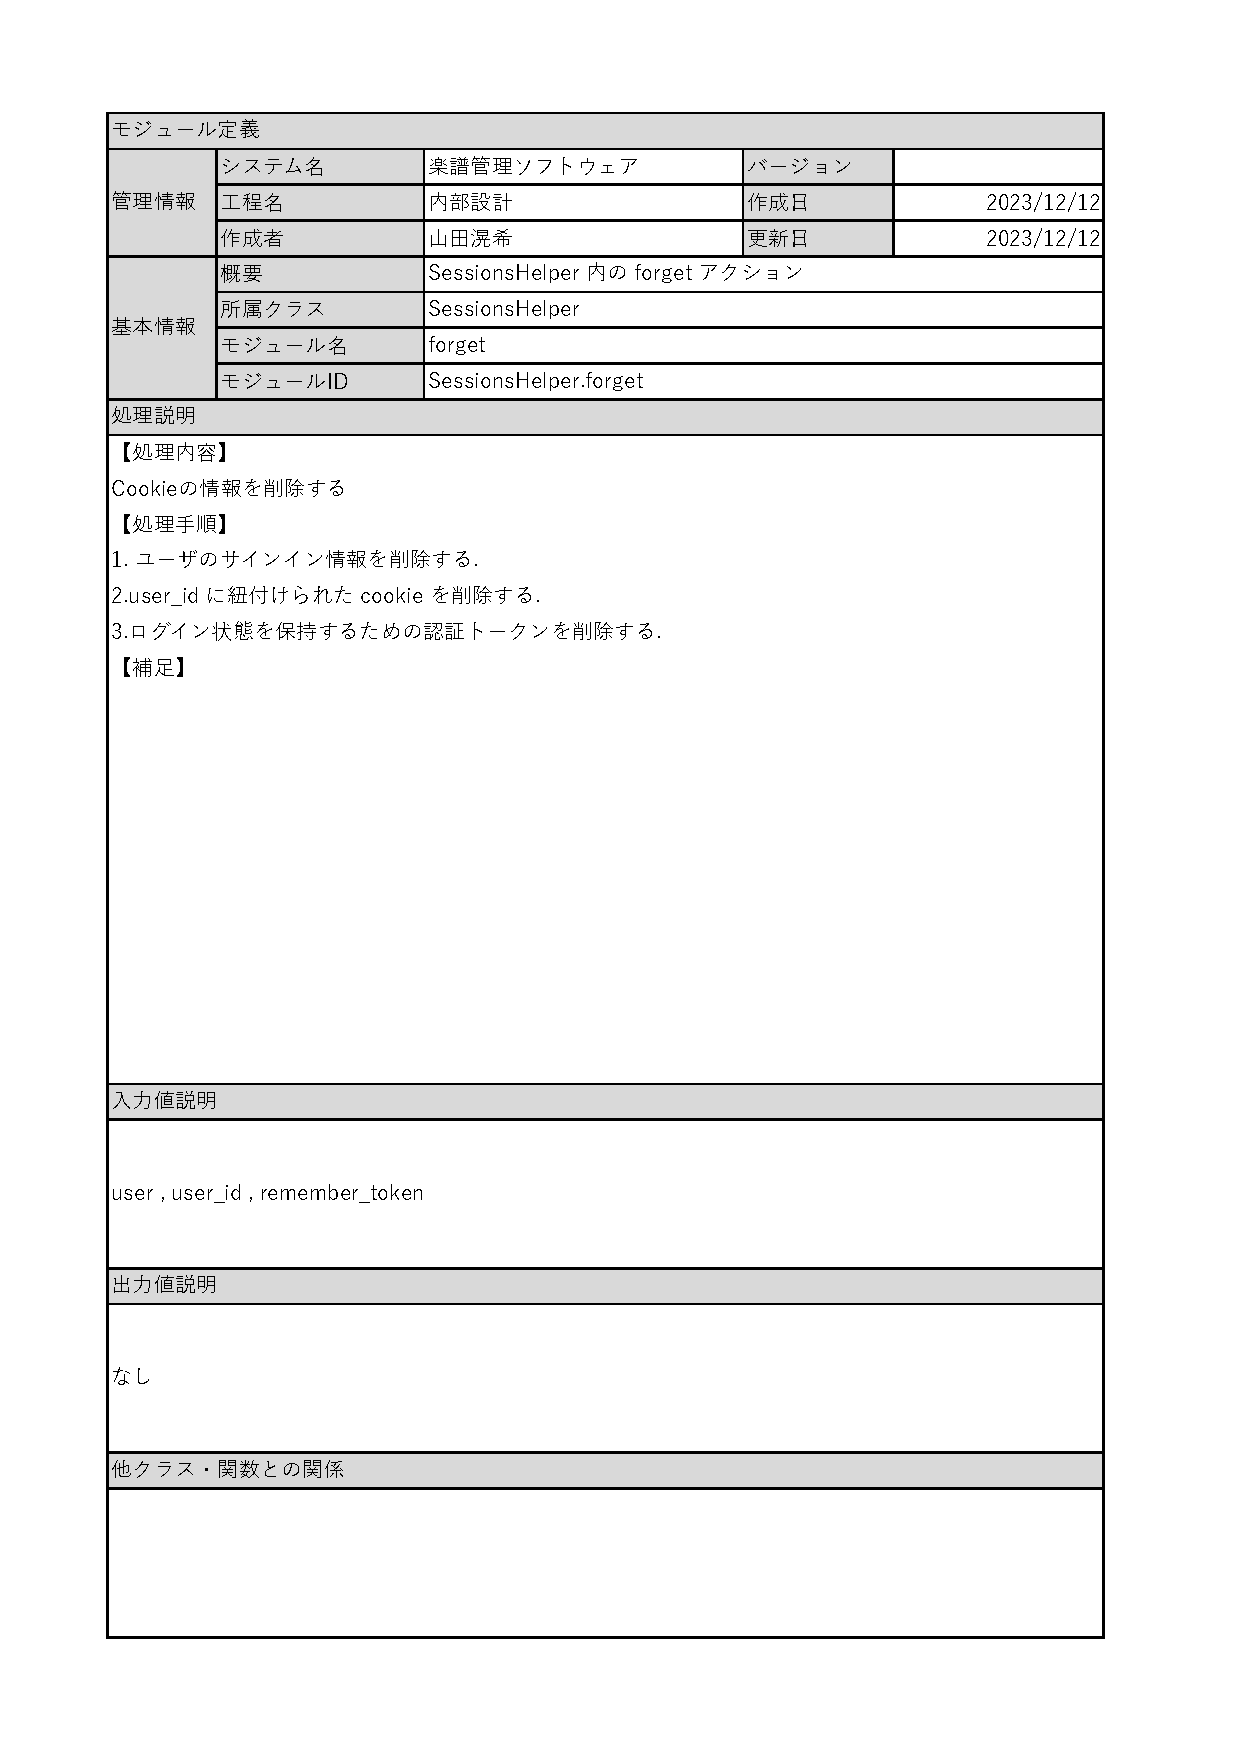
\includegraphics[scale=0.5]{img/Helper/SessionsHelper_forget.pdf}
    \caption{SessionsHelper.forget}
\end{figure}
\clearpage

%url保存
\subsection*{アクセスしようとしたurlを保存する機能}
リダイレクト時にエラーが起こったとき,直前のページへ戻るために使用される.
\begin{figure}[H]
    \centering
    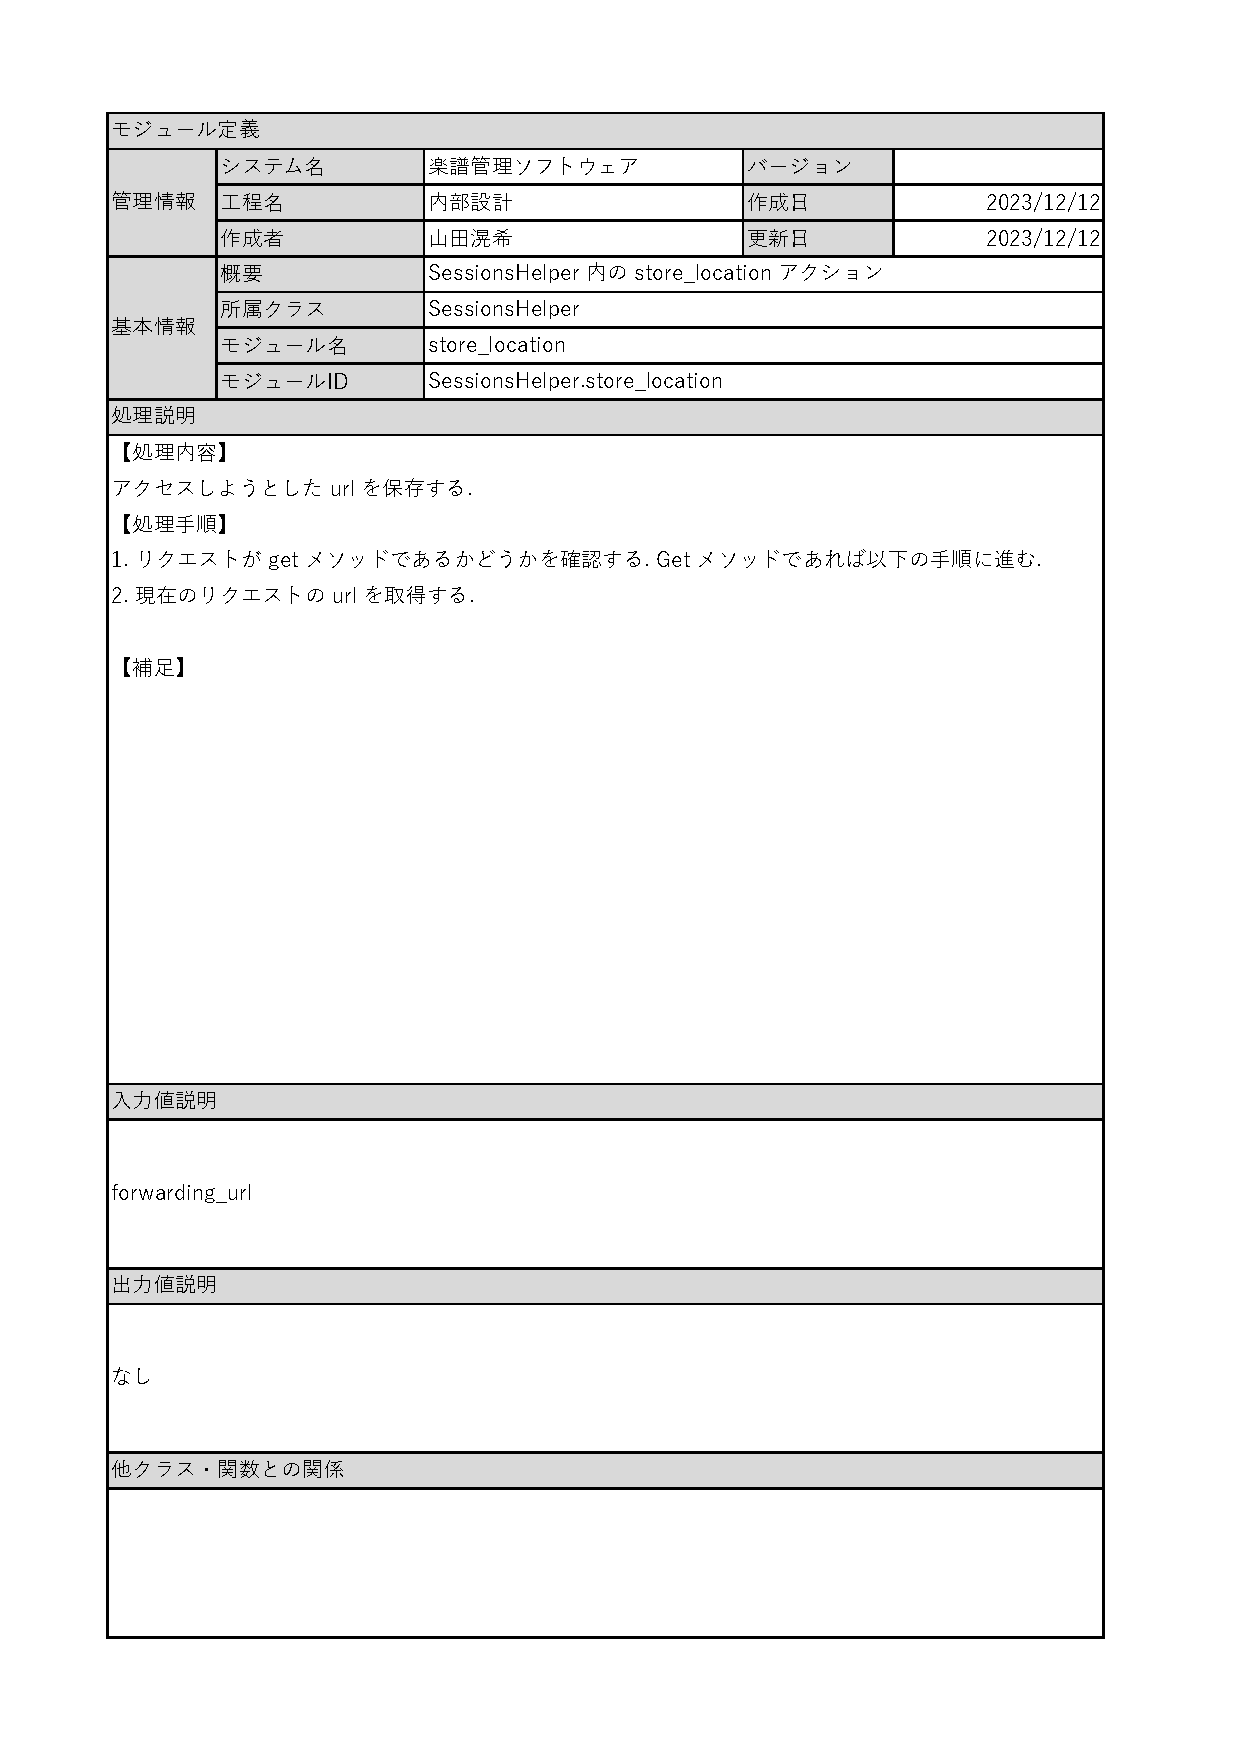
\includegraphics[scale=0.5]{img/Helper/SessionsHelper_store_location.pdf}
    \caption{SessionsHelper.store\_location}
\end{figure}
\clearpage

%ユーザ判定
\subsection*{管理者,ユーザを判定する機能}
管理者かどうかの判定,またログイン中のユーザかの判定に使用される.
\begin{figure}[H]
    \centering
    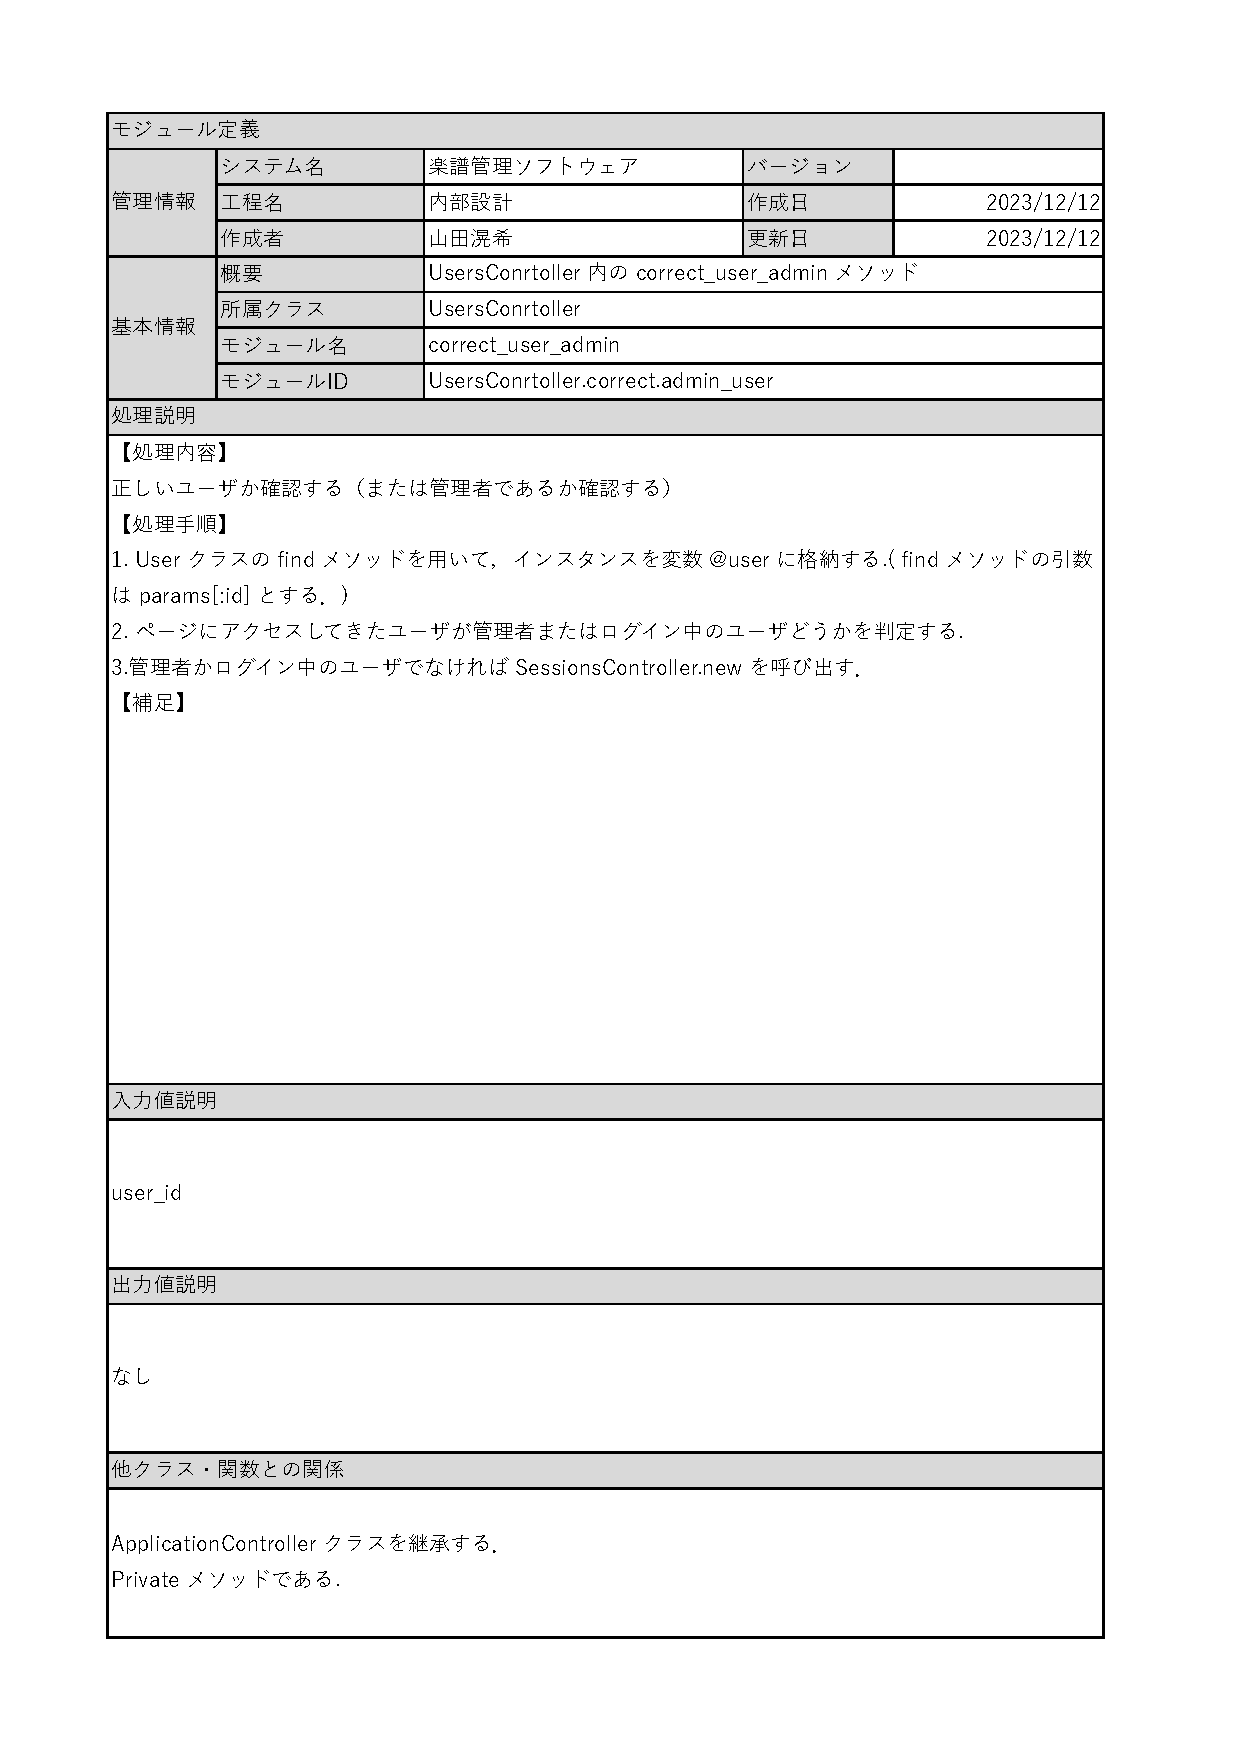
\includegraphics[scale=0.5]{img/Method/UsersController_correct_user_admin.pdf}
    \caption{UsersController.correct\_user\_admin}
\end{figure}
\clearpage

%管理者判定
\subsection*{管理者の判定機能}
題の通り.
\begin{figure}[H]
    \centering
    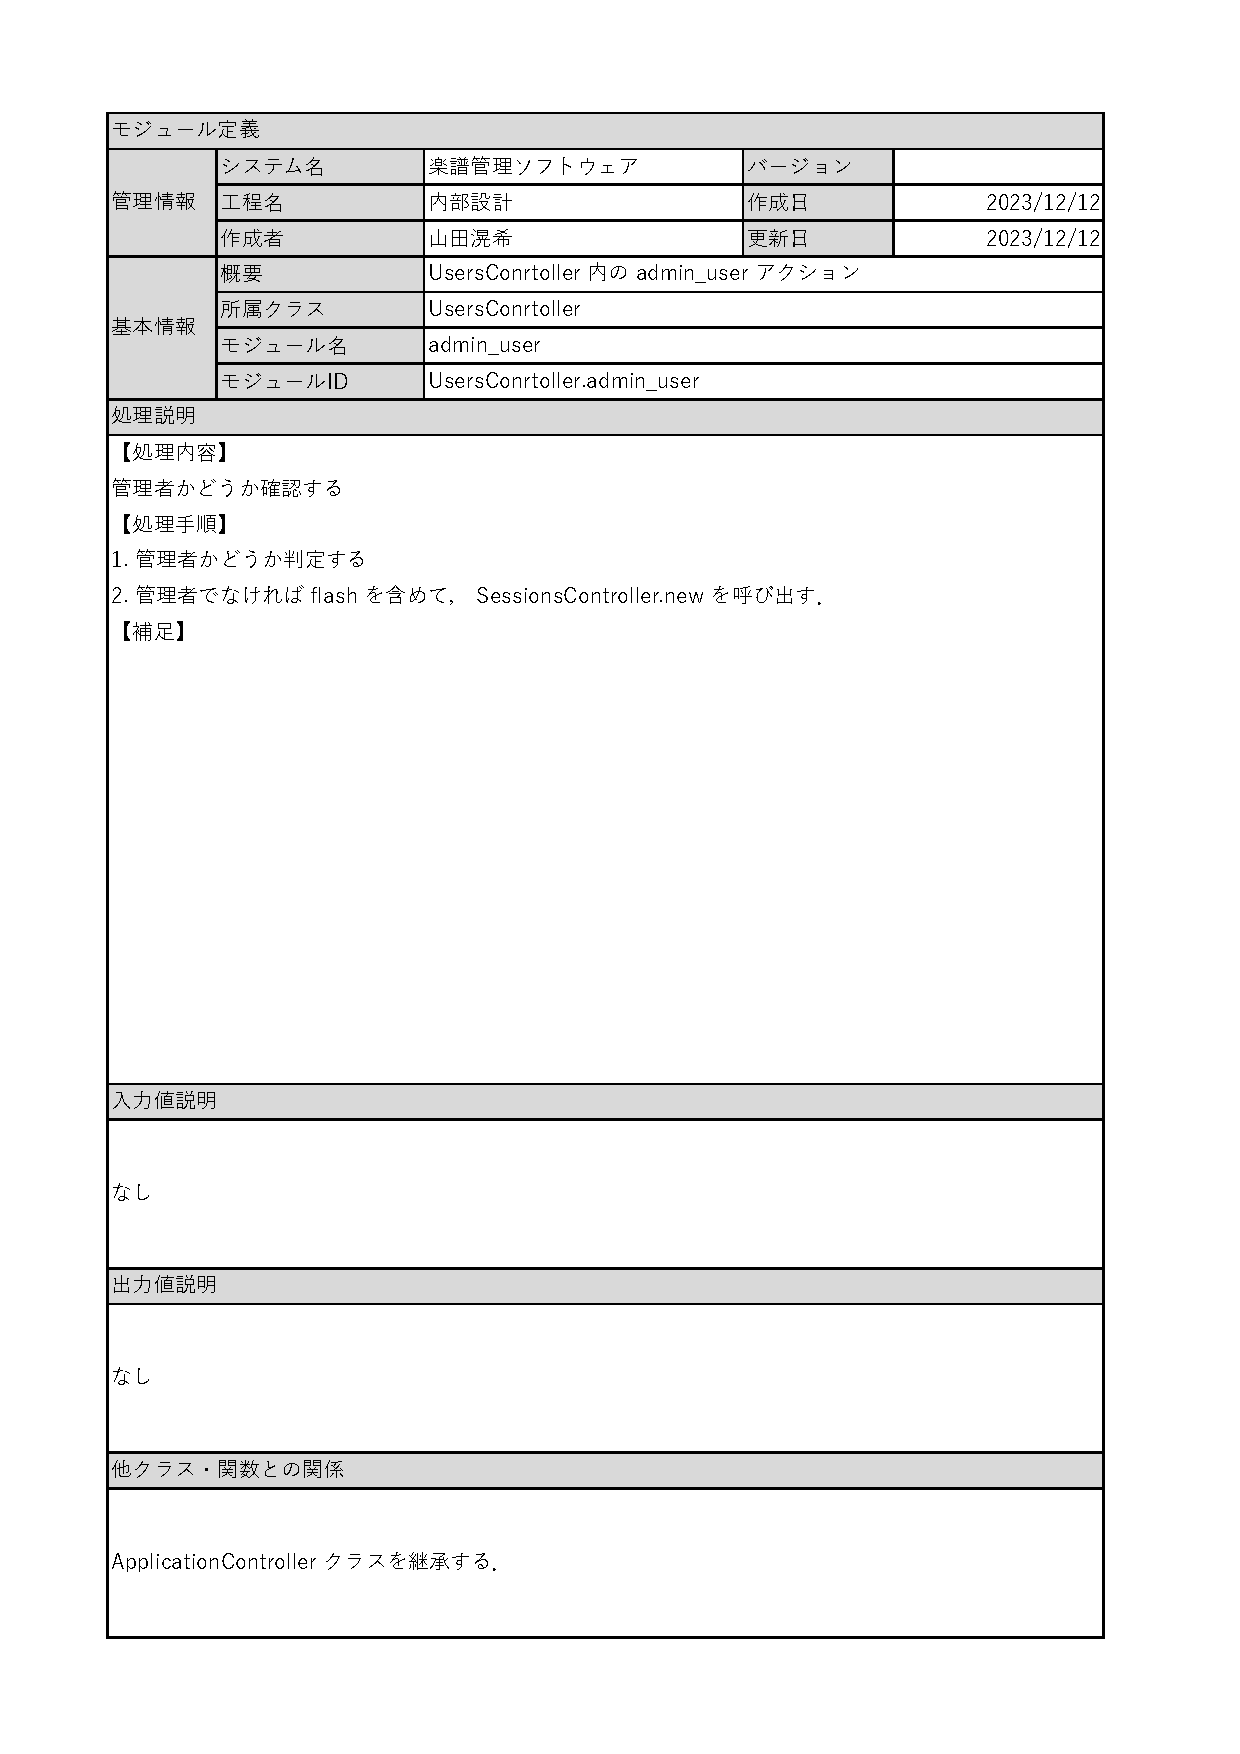
\includegraphics[scale=0.5]{img/Method/UsersController_admin_user.pdf}
    \caption{UsersController.admin\_user}
\end{figure}
\clearpage

%入力値取得
\subsection*{登録・編集入力取得機能}
ScoresController.new,ScoresController.edit,UsersController.new,UsersController.edit
のViewへの入力値取得に使用される.
\begin{figure}[H]
    \centering
    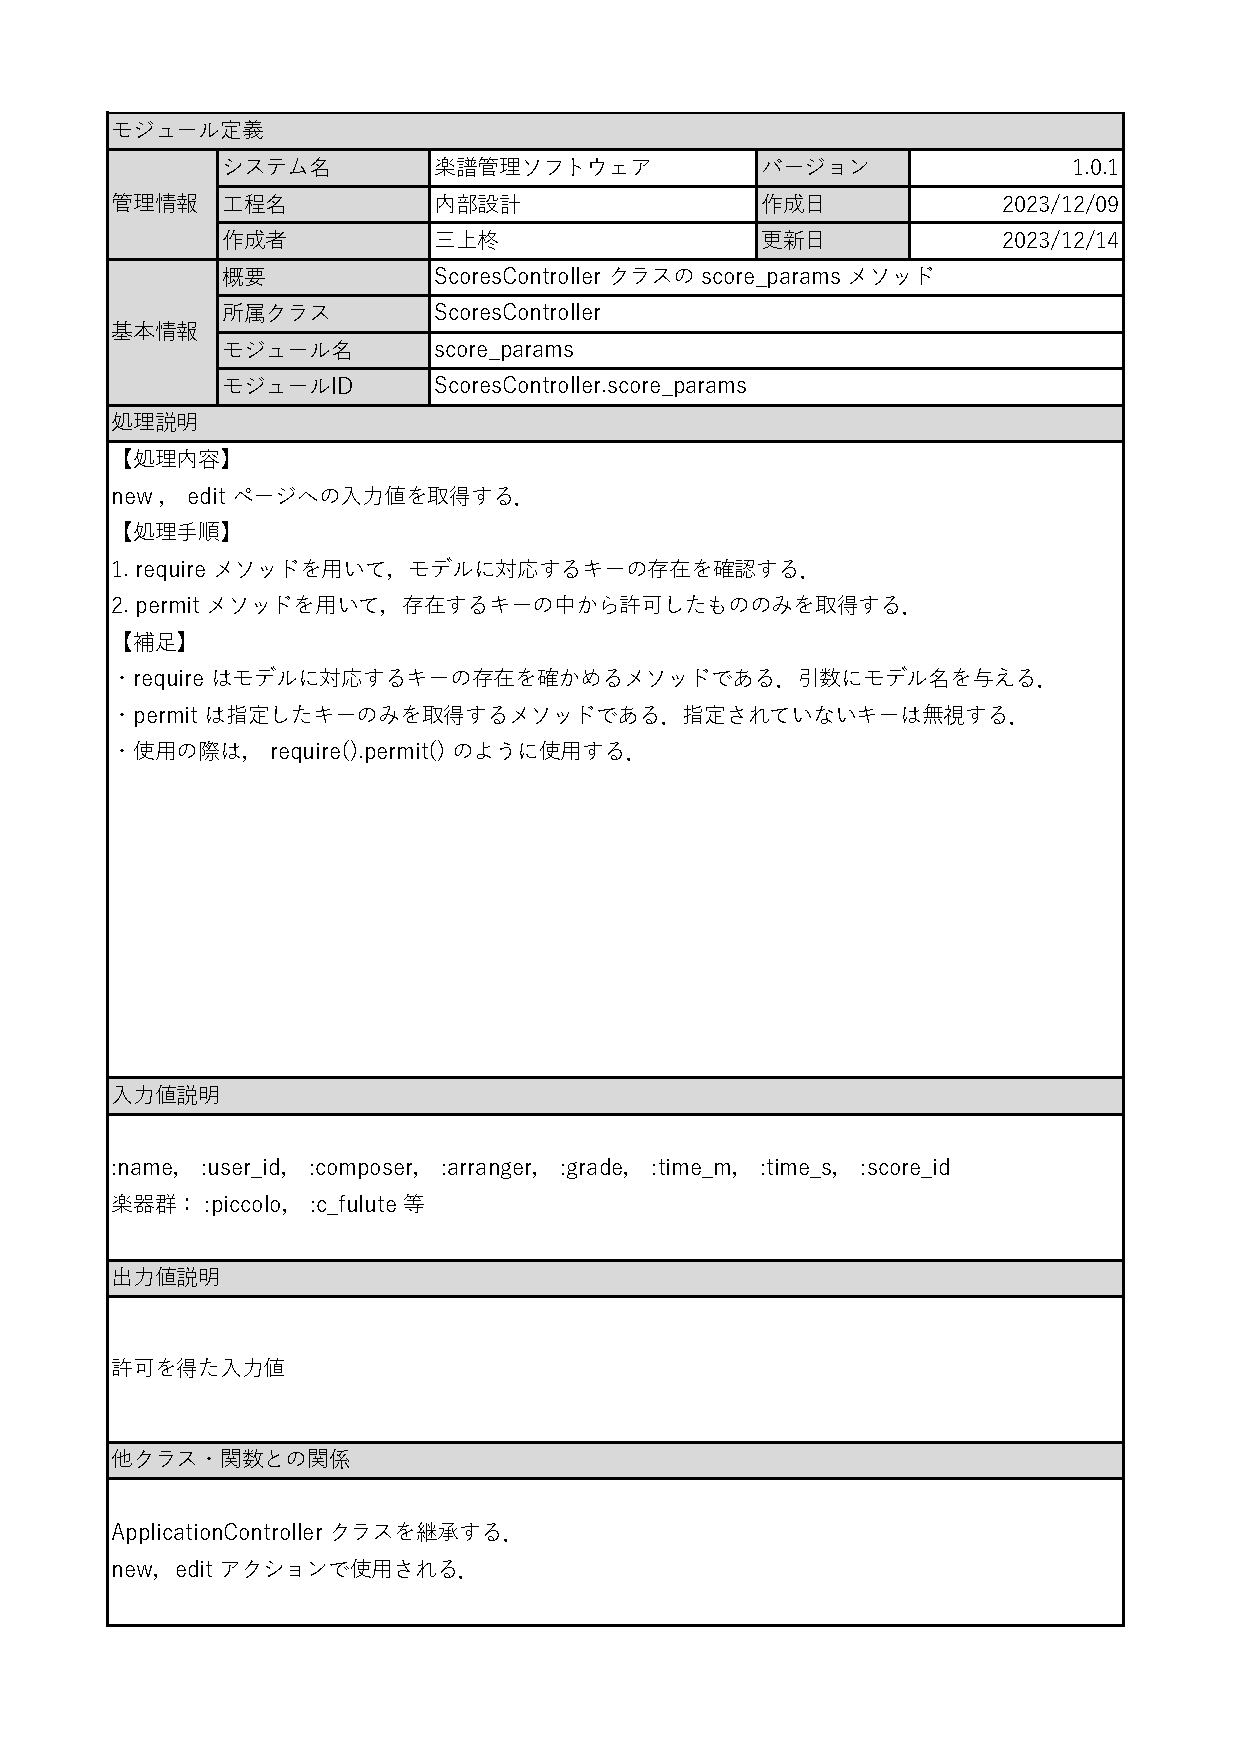
\includegraphics[scale=0.5]{img/Method/score_params.pdf}
    \caption{ScoresController.score\_params}
\end{figure}
\begin{figure}
    \centering
    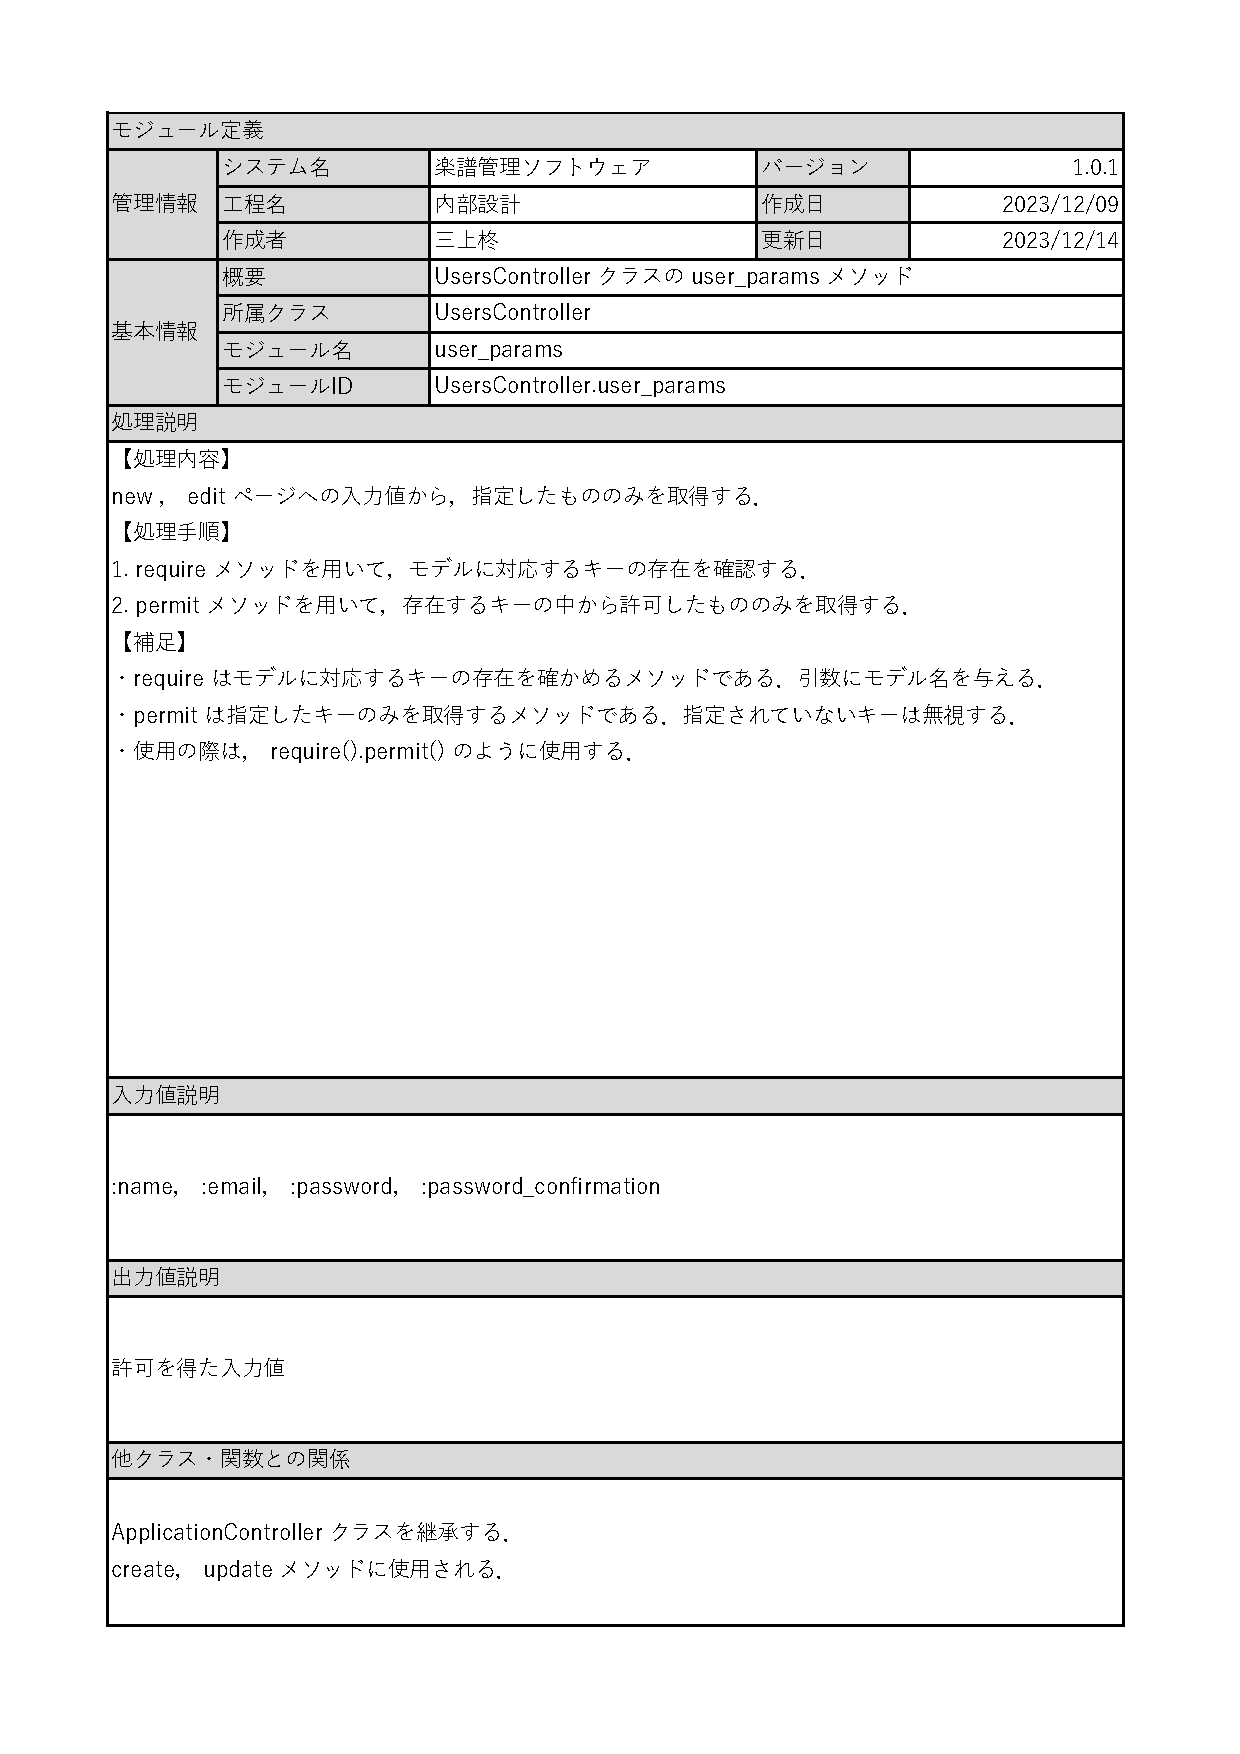
\includegraphics[scale=0.5]{img/Method/user_params.pdf}
    \caption{UsersController.user\_params}
\end{figure}
\clearpage

%ログアウト
\subsection*{ログアウト機能}
ログアウトに使用される.ユーザがログイン状態でなくなる.
\begin{figure}[H]
    \centering
    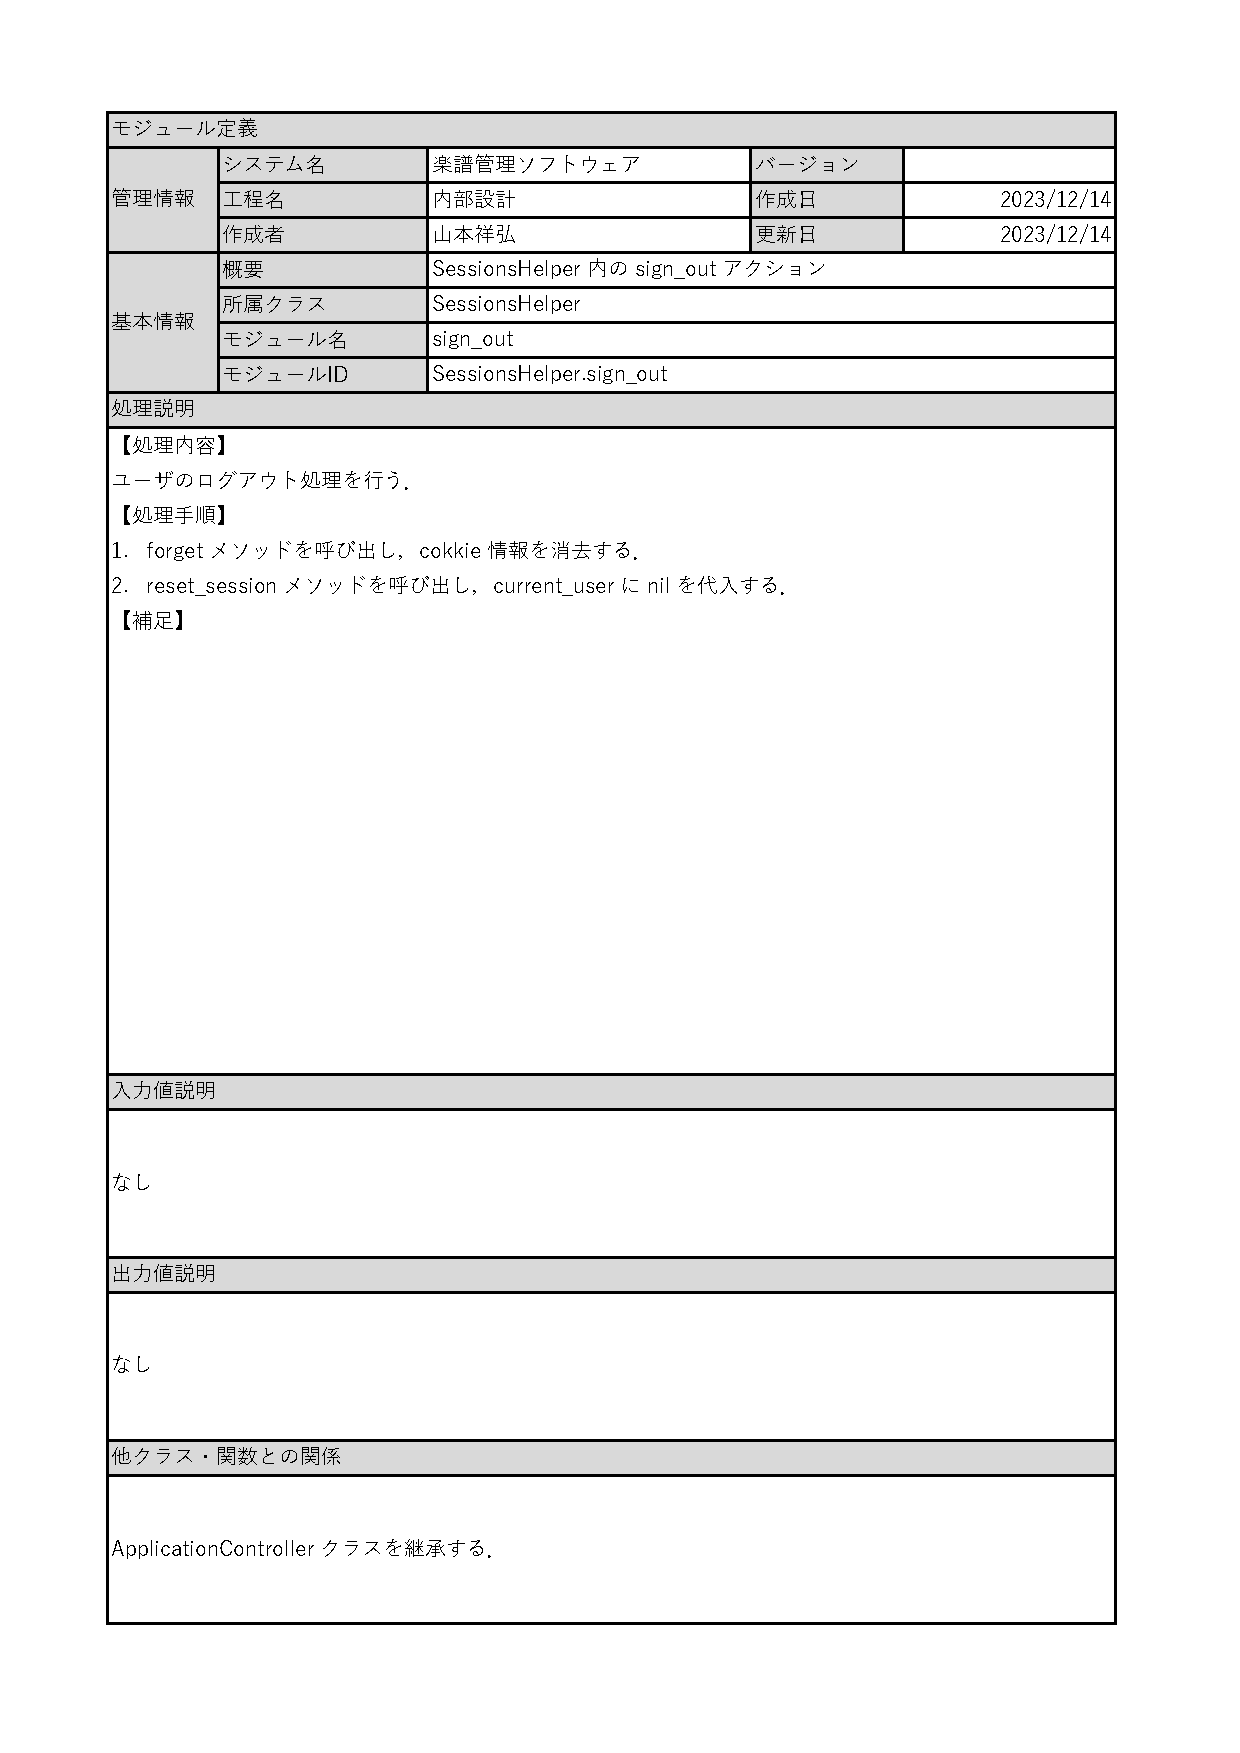
\includegraphics[scale=0.5]{img/Helper/SessionsHelper.sign_out.pdf}
    \caption{SessionsHelper.sign\_out}
\end{figure}
\clearpage

\section{モデル}
モデルに記述する正規表現等はメソッドと呼ばないことから,別に記述する.
\begin{figure}[H]
    \centering
    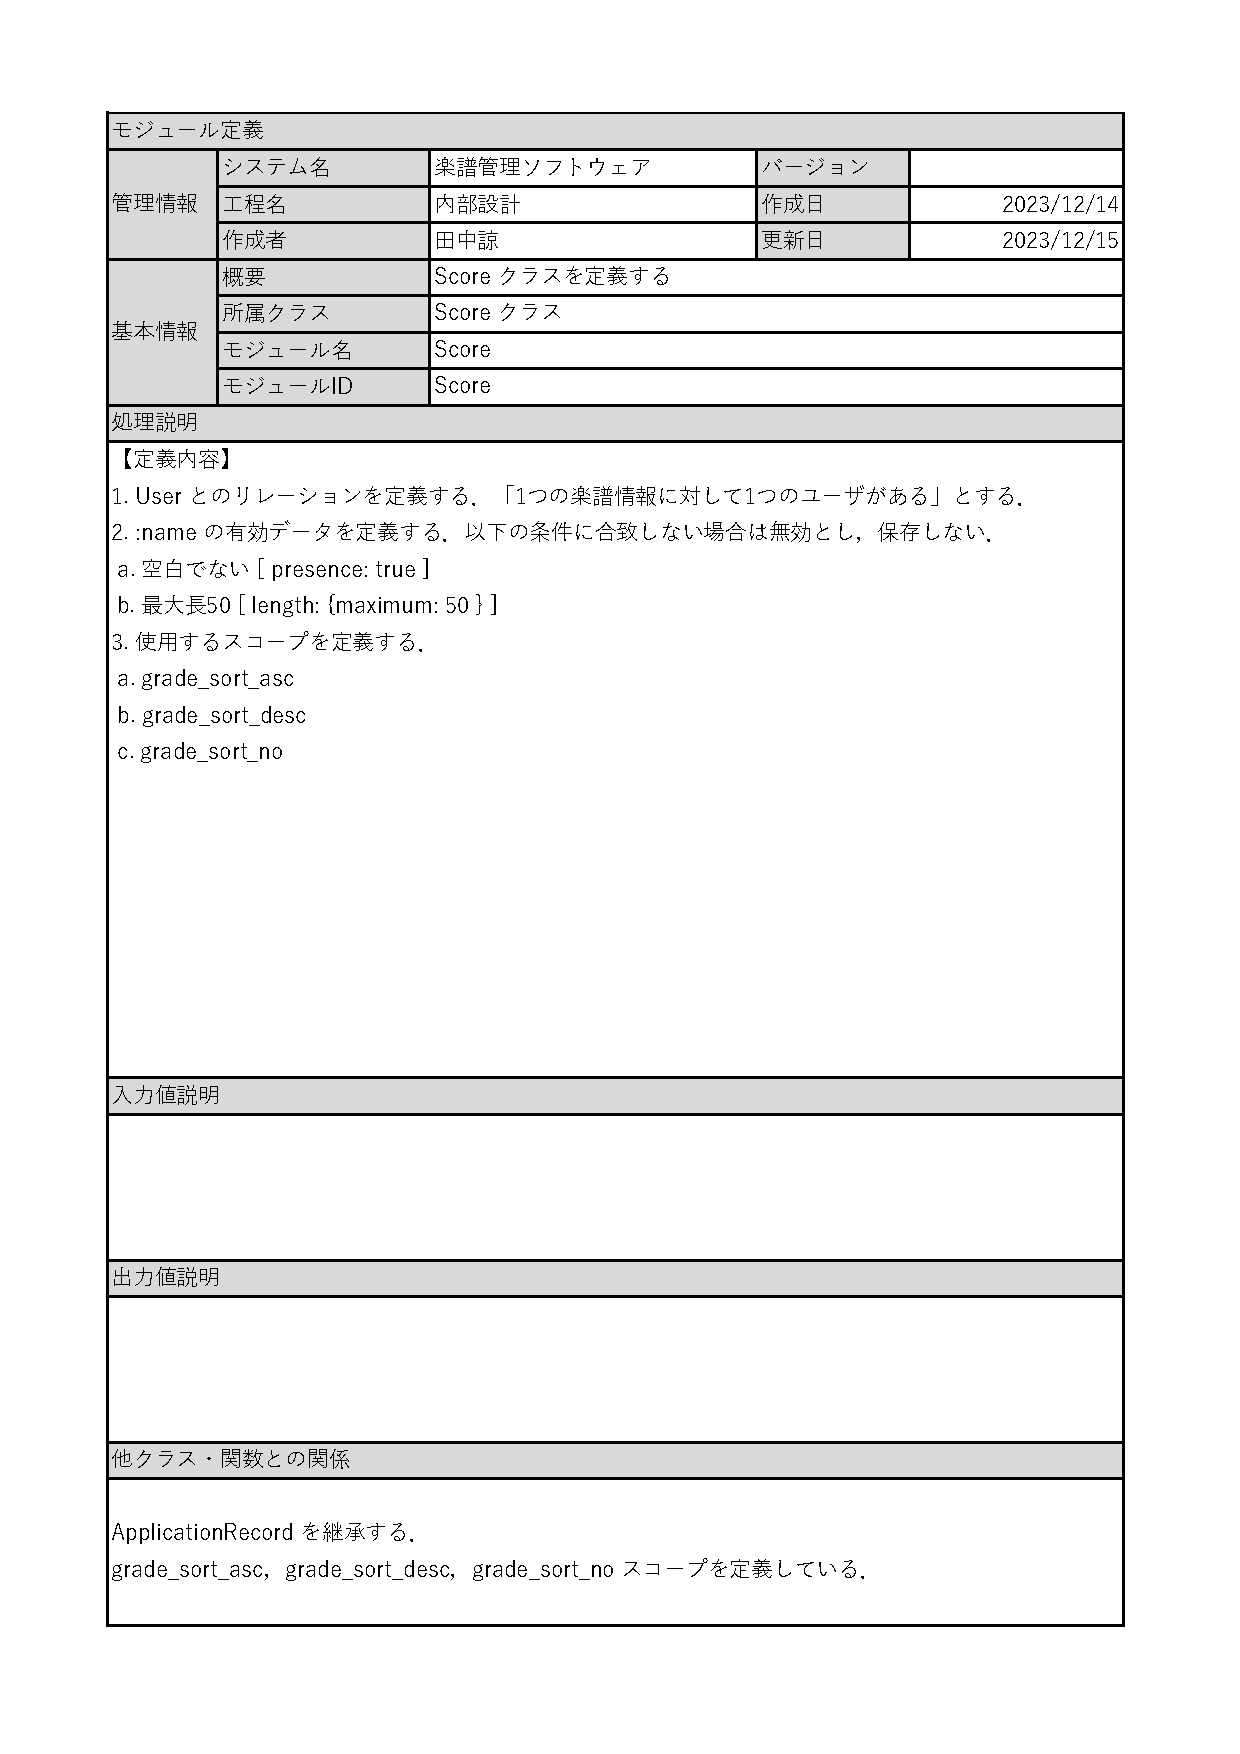
\includegraphics[scale=0.5]{img/Model/Score.pdf}
    \caption{Score}
\end{figure}
\begin{figure}
    \centering
    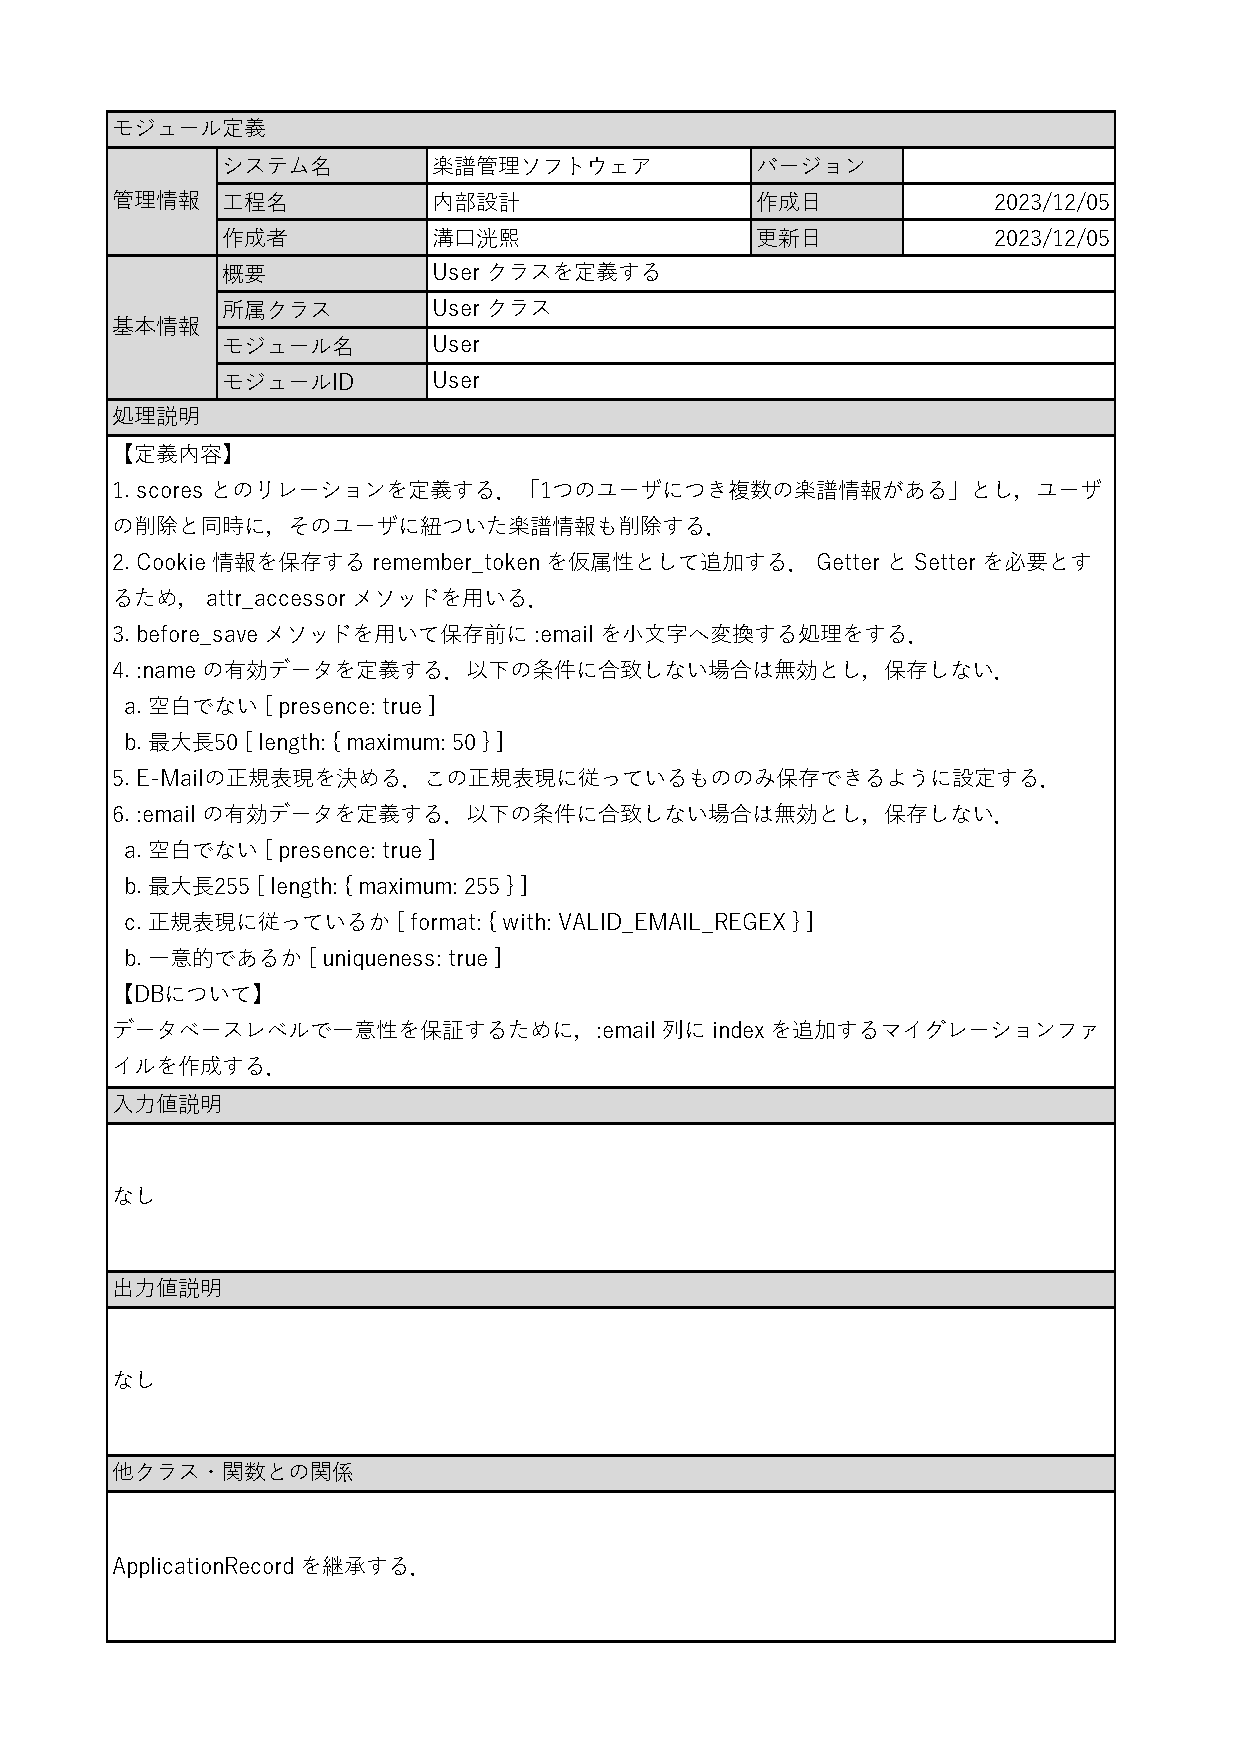
\includegraphics[scale=0.5]{img/Model/User.pdf}
    \caption{User}
\end{figure}